% % Preamble BEGINN %%%%%%%%%%%%%%%%%%%%%%%%%%%%%%%%%%%%%%%%%%%%%%%%%%%%%%%%%

%%% Preamble (Dokumentenklasse)
% ------------------------------------------------------------------------
% LaTeX - Preambel ******************************************************
% ------------------------------------------------------------------------
% Dokumentklasse (Koma Script)
% ------------------------------------------------------------------------
% basiernd auf www.matthiaspospiech.de/latex/vorlagen Diplomarbeit kompakt
% ========================================================================
\documentclass[%
   %draft,            % Entwurfsstadium
   final,             % fertiges Dokument
   12pt,              % Schriftgroesse der Grundschrift
   bigheadings,       % gro�e �berschriften
   ngerman,           % wird an andere Pakete weitergereicht
   a4paper,           % Papierformat
   BCOR5mm,          % Bindekorrektur: Zus�tzlicher Rand auf der Innenseite
   DIV14,            % Seitengr��e (siehe Koma Skript Dokumentation !)
   1.1headlines,     % Zeilenanzahl der Kopfzeilen
   pagesize,         % Schreibt die Papiergroesse in die Datei.
   oneside,          % Einseitiges Layout
%   twoside,          % Zweiseitiges Layout
   openright,        % Kapitel beginnen immer auf der rechten Seite
   titlepage,        % Titel als einzelne Seite ('titlepage' Umgebung)  
   headsepline,      % Linie unter Kolumnentitel ()
   footsepline,		 % Linie �ber Seitenzahl
%   plainheadsepline, % Linie unter Kolumnentitel () plain Seitenstil
   nochapterprefix,  % keine Ausgabe von 'Kapitel:'
   bibtotoc,         % Bibliographie ins TOC
%	bibtotocnumbered, % Bibliographie ins TOC mit Kapitelnummer
   tocindent,        % eingereuckte Gliederung
   listsindent,      % eingereuckte LOT, LOF
   pointlessnumbers, % �berschriftnummerierung ohne Punkt, siehe DUDEN !
   cleardoubleempty, % Leere linke Seite bei Zweiseitenlayout vor Kapitel
   fleqn,            % Formeln werden linksbuendig angezeigt
%   parindent,        % Absatz mit Einzug (Standard)
   halfparskip,      % Absatz halbe Zeile Abstand
%   parskip,          % Absatz ganze Zeile Abstand
]{scrbook}%     Klassen: scrartcl, scrreprt, scrbook


%%% Alle Namen usw. im Titel und im hyperref-Paket
% ------------------------------------------------------------------------
% LaTeX - Preambel ******************************************************
% ------------------------------------------------------------------------
% pre-work
% ========================================================================
% % ToDo kennzeichnen
\newcommand{\workTodo}[1]{\textcolor{red}{todo: #1}}

% % F�r Datum und Zeit in Fusszeile
% % !!!Inhalt bei Fertigstellung der Arbeit l�schen
\newcommand{\workMarkDateTime}{\workTodo{\today{} - \thistime\ Uhr}}

% % Alle Namen werden im Titel und im hyperref-Paket eingetragen
% % !!! Ueberall f�r <Wert> das Entsprechende eintragen

 % <Typ> Studienarbeit, Dipolmarbeit, Studienarbeit oder Bachlor-Abschlussarbeit
\newcommand{\workTyp}{Assignment\xspace}

 % <Titel> der Arbeit
\newcommand{\workTitel}{PCM}

 % <Studiengang> z.B. Kommunikationstechnik
\newcommand{\workStudiengang}{Technische Informatik\xspace}

% <Semester> mit Jahr z.B. Sommersemester 2008  
\newcommand{\workSemester}{Sommersemester 2017\xspace}

% <Name> des Studenten
\newcommand{\workNameStudent}{Antonio Parrotta\xspace}

% <Pruefer> Name des pr�fenden (betreuenden) Professor an der Hochschule
\newcommand{\workPruefer}{Dr. x\xspace} 


% %%% Nur bei Abschluss-Arbeiten

% <Datum> der Abgabe der Arbeit (Eidesstatliche Erkl�rung)
\newcommand{\workDatum}{\today\xspace}

% <Zweitpr�fer>
\newcommand{\workZweitPruefer}{Dipl.-Ing. xy \xspace}

% %%% Nur bei Industrie-Arbeiten:

% <Firma>
\newcommand{\workFirma}{IT-Designers GmbH\xspace}

% Firmenlogo Name hier anpassen, Gr��e (wenn m�glich) nicht �ndern
%\newcommand{\workFirmenLogo}{\includegraphics[width=5cm]{fig/aa-titel/Bosch_4C_S}} 


%%% Preamble (Pakete)
% ------------------------------------------------------------------------
% LaTeX - Preambel ******************************************************
% ------------------------------------------------------------------------
% Packages
% ------------------------------------------------------------------------
% basiernd auf www.matthiaspospiech.de/latex/vorlagen Diplomarbeit kompakt
% ========================================================================

% Inhalt:
% 1. Einige Pakete muessen unbedingt vor allen anderen geladen werden
% 2. Fonts Fonts Fonts
% 3. Math Packages
% 4. Symbole
% 5. text related packages
% 6. Pakete zum Zitieren
% 7. PDF related packages
% 8. Tables (Tabular)
% 9. figures and placement
% 10. verbatim packages
% 11. science packages
% 12. layout packages

% ~~~~~~~~~~~~~~~~~~~~~~~~~~~~~~~~~~~~~~~~~~~~~~~~~~~~~~~~~~~~~~~~~~~~~~~~
% Encoding der Dateien (sonst funktionieren Umlaute nicht)
% Empfohlen latin1, da einige Pakete mit utf8 Zeichen nicht
% funktionieren, z.B: listings, soul.

\usepackage[latin1]{inputenx} % ISO-8859-1
%\usepackage[ansinew]{inputenx} % Windows-Standard (CP1252) (baut auf ISO 8859-1 und ISO 8859-15 auf)
%\usepackage[utf8]{inputenc}

% ~~~~~~~~~~~~~~~~~~~~~~~~~~~~~~~~~~~~~~~~~~~~~~~~~~~~~~~~~~~~~~~~~~~~~~~~
% 1. Einige Pakete muessen unbedingt vor allen anderen geladen werden
% ~~~~~~~~~~~~~~~~~~~~~~~~~~~~~~~~~~~~~~~~~~~~~~~~~~~~~~~~~~~~~~~~~~~~~~~~
%
\usepackage{xspace} % Define commands that don't eat spaces.
\usepackage{ifpdf} % Fuer Pakete/Paketoptionen, die nur fuer pdf benoetigt werden \ifpdf \else \fi
\usepackage{calc} % Calculation with LaTeX
\usepackage[english, ngerman]{babel} % Languagesetting
\usepackage[table]{xcolor} % Farben
\usepackage[]{graphicx} % Bilder
\usepackage{subfig}
%\usepackage{epstopdf} % If an eps image is detected, epstopdf is automatically called to convert it to pdf format.
\usepackage[]{amsmath} % Amsmath - Mathematik Basispaket
\usepackage{ragged2e} % Besserer Flatternsatz (Linksbuendig, statt Blocksatz)

% ~~~~~~~~~~~~~~~~~~~~~~~~~~~~~~~~~~~~~~~~~~~~~~~~~~~~~~~~~~~~~~~~~~~~~~~~
% 2. Fonts Fonts Fonts
% ~~~~~~~~~~~~~~~~~~~~~~~~~~~~~~~~~~~~~~~~~~~~~~~~~~~~~~~~~~~~~~~~~~~~~~~~

\usepackage[T1]{fontenc} % T1 Schrift Encoding (notwendig f�r die meisten Type 1 Schriften)
\usepackage{textcomp}	 % Zusatzliche Symbole (Text Companion font extension)

% Alle Schriften die hier angegeben sind sehen im PDF richtig aus.
% Die LaTeX Standardschrift ist die Latin Modern (lmodern Paket).
% If Latin Modern is not available for your distribution you must install the
% package cm-super instead. Otherwise your fonts will look horrible in the PDF

% DO NOT LOAD ae-Package for the font !

%% - Latin Modern
\usepackage{lmodern}
%% -------------------
%
% % - Times, Helvetica, Courier (Word Standard...)
%\usepackage{mathptmx}
%\usepackage[scaled=.90]{helvet}
%\usepackage{courier}
% % -------------------
%%
%% - Palantino , Helvetica, Courier
%\usepackage{mathpazo}
%\usepackage[scaled=.95]{helvet}
%\usepackage{courier}
%% -------------------
%
%% - Bera Schriften
%\usepackage{bera}
%% -------------------
%
%% - Charter, Bera Sans
%\usepackage{charter}\linespread{1.05}
%\renewcommand{\sfdefault}{fvs}


% ~~~~~~~~~~~~~~~~~~~~~~~~~~~~~~~~~~~~~~~~~~~~~~~~~~~~~~~~~~~~~~~~~~~~~~~~
% 3. Math Packages
% ~~~~~~~~~~~~~~~~~~~~~~~~~~~~~~~~~~~~~~~~~~~~~~~~~~~~~~~~~~~~~~~~~~~~~~~~

\usepackage[fixamsmath,disallowspaces]{mathtools} % Erweitert amsmath und behebt einige Bugs
\usepackage{fixmath}
\usepackage[all,warning]{onlyamsmath} % Warnt bei Benutzung von Befehlen die mit amsmath inkompatibel sind.
\usepackage{icomma} % Erlaubt die Benutzung von Kommas im Mathematikmodus

% ~~~~~~~~~~~~~~~~~~~~~~~~~~~~~~~~~~~~~~~~~~~~~~~~~~~~~~~~~~~~~~~~~~~~~~~~
% 4. Symbole
% ~~~~~~~~~~~~~~~~~~~~~~~~~~~~~~~~~~~~~~~~~~~~~~~~~~~~~~~~~~~~~~~~~~~~~~~~
\usepackage{amssymb}
\usepackage{eurosym}
%\usepackage{wasysym}
%\usepackage{marvosym}
%\usepackage{pifont}

% ~~~~~~~~~~~~~~~~~~~~~~~~~~~~~~~~~~~~~~~~~~~~~~~~~~~~~~~~~~~~~~~~~~~~~~~~
% 5. text related packages
% ~~~~~~~~~~~~~~~~~~~~~~~~~~~~~~~~~~~~~~~~~~~~~~~~~~~~~~~~~~~~~~~~~~~~~~~~

\usepackage{url} % Setzen von URLs. In Verbindung mit hyperref sind diese auch aktive Links.
\usepackage[stable,perpage, ragged,  multiple]{footmisc} % Fussnoten
\usepackage[ngerman]{varioref} % Intelligente Querverweise
\usepackage{enumitem} % Listen
\usepackage{framed}
\usepackage{lscape}
\usepackage{geometry}

\def\UrlBreaks{\do\/\do-}
% ~~~~~~~~~~~~~~~~~~~~~~~~~~~~~~~~~~~~~~~~~~~~~~~~~~~~~~~~~~~~~~~~~~~~~~~~
% 6. Pakete zum Zitieren
% ~~~~~~~~~~~~~~~~~~~~~~~~~~~~~~~~~~~~~~~~~~~~~~~~~~~~~~~~~~~~~~~~~~~~~~~~

\usepackage[babel, german=quotes, english=british, french=guillemets]{csquotes} % clever quotations
\SetBlockThreshold{2} % Anzahl von Zeilen
\newenvironment{myquote}%
          {\begin{quote}\small}%
          {\end{quote}}%
\SetBlockEnvironment{myquote}
\usepackage{nameref}

% ~~~~~~~~~~~~~~~~~~~~~~~~~~~~~~~~~~~~~~~~~~~~~~~~~~~~~~~~~~~~~~~~~~~~~~~~
% 7. PDF related packages
% ~~~~~~~~~~~~~~~~~~~~~~~~~~~~~~~~~~~~~~~~~~~~~~~~~~~~~~~~~~~~~~~~~~~~~~~~

\ifpdf % Wenn als PDF ausgegeben wird
\usepackage{pdfpages} % pdf-Seiten einbinden
\usepackage[pdftex]{hyperref} % PDF Option in Hyperref
\else
\usepackage[dvipdfm]{hyperref}
\fi

%%% Doc: ftp://tug.ctan.org/pub/tex-archive/macros/latex/contrib/pdfpages/pdfpages.pdf
%\usepackage{pdfpages} % Include pages from external PDF documents in LaTeX documents

%%% Doc: ftp://tug.ctan.org/pub/tex-archive/macros/latex/contrib/hyperref/doc/manual.pdf
\hypersetup{
          pdfhighlight = /O,	         % Visualisierung beim anklicken von Links
% Farben fuer die Links
   colorlinks=true,	        % Links erhalten Farben statt Kaestchen
   urlcolor=darkblue,    % \href{...}{...} external (URL)
   filecolor=darkblue,  % \href{...} local file
   linkcolor=darkblue,  % \ref{...} and \pageref{...}
          citecolor =darkblue,    % Literaturverzeichnis
   % Links
   raiselinks=true,			 % calculate real height of the link
   breaklinks=true,	        % Links bestehen bei Zeilenumbruch
%   backref=page,	         % Backlinks im Literaturverzeichnis (section, slide, page, none)
%   pagebackref=true,        % Backlinks im Literaturverzeichnis mit Seitenangabe
   verbose,
%   hyperindex=true,         % backlinkex index
   linktocpage=true,        % Inhaltsverzeichnis verlinkt Seiten
%   hyperfootnotes=false,	% Keine Links auf Fussnoten
   % Bookmarks
%   bookmarks=true,	         % Erzeugung von Bookmarks fuer PDF-Viewer
   bookmarksopenlevel=1,    % Gliederungstiefe der Bookmarks
   bookmarksopen=true,      % Expandierte Untermenues in Bookmarks
   bookmarksnumbered=true,  % Nummerierung der Bookmarks
   bookmarkstype=toc,       % Art der Verzeichnisses
   % Anchors
   plainpages=false,        % % Make page anchors using the formatted form of the page number. With this option, hyperref writes different anchors for pages �ii� and �2�. (If the option is set �true� � the default � hyperref writes page anchors as the arabic form of the absolute page number, rather than the formatted form.)
   % hypertexnames=false,
   pageanchor=true,	        % Pages are linkable
   % PDF Informationen
   pdftitle={\workTyp: \workTitel},	        % Titel
   pdfauthor={\workNameStudent},	    % Autor
   pdfcreator={LaTeX, hyperref, KOMA-Script}, % Ersteller
   %pdfproducer={pdfeTeX 1.10b-2.1} %Produzent
   pdfstartview=FitH,       % Dokument wird Fit Width geaefnet
   pdfpagemode=UseOutlines, % Bookmarks im Viewer anzeigen
%   pdfpagelabels=true,      % set PDF page labels
}

% ~~~~~~~~~~~~~~~~~~~~~~~~~~~~~~~~~~~~~~~~~~~~~~~~~~~~~~~~~~~~~~~~~~~~~~~~
% 8. Tables (Tabular)
% ~~~~~~~~~~~~~~~~~~~~~~~~~~~~~~~~~~~~~~~~~~~~~~~~~~~~~~~~~~~~~~~~~~~~~~~~

\usepackage{booktabs}
\usepackage{tabularx} % tabularx nach hyperref laden
\usepackage{multirow}

% ~~~~~~~~~~~~~~~~~~~~~~~~~~~~~~~~~~~~~~~~~~~~~~~~~~~~~~~~~~~~~~~~~~~~~~~~
% 9. figures and placement
% ~~~~~~~~~~~~~~~~~~~~~~~~~~~~~~~~~~~~~~~~~~~~~~~~~~~~~~~~~~~~~~~~~~~~~~~~

%% Bilder und Graphiken ==================================================

\usepackage{float}	% Stellt die Option [H] fuer Floats zur Verfgung
\usepackage{flafter} % Floats immer erst nach der Referenz setzen
\usepackage{subfig} % Layout wird weiter unten festgelegt !
\usepackage{wrapfig} % Bilder von Text Umfliessen lassen

\usepackage{placeins} % Alle Floats bis \FloatBarrier ausgeben

% Make float placement easier
\renewcommand{\floatpagefraction}{.75} % vorher: .5
\renewcommand{\textfraction}{.1}       % vorher: .2
\renewcommand{\topfraction}{.8}        % vorher: .7
\renewcommand{\bottomfraction}{.5}     % vorher: .3
\setcounter{topnumber}{3}	         % vorher: 2
\setcounter{bottomnumber}{2}	         % vorher: 1
\setcounter{totalnumber}{5}	         % vorher: 3


% ~~~~~~~~~~~~~~~~~~~~~~~~~~~~~~~~~~~~~~~~~~~~~~~~~~~~~~~~~~~~~~~~~~~~~~~~
% 10. verbatim packages
% ~~~~~~~~~~~~~~~~~~~~~~~~~~~~~~~~~~~~~~~~~~~~~~~~~~~~~~~~~~~~~~~~~~~~~~~~

%%% Doc: ftp://tug.ctan.org/pub/tex-archive/macros/latex/contrib/upquote/upquote.sty
\usepackage{upquote} % Setzt "richtige" Quotes in verbatim-Umgebung

%%% Doc: No Documentation
% \usepackage{verbatim} % Reimplemntation of the original verbatim

%%% Doc: http://www.cs.brown.edu/system/software/latex/doc/fancyvrb.pdf
% \usepackage{fancyvrb} % Superior Verbatim Class

%% Listings Paket ------------------------------------------------------
%%% Doc: ftp://tug.ctan.org/pub/tex-archive/macros/latex/contrib/listings/listings-1.3.pdf
\usepackage{listings}

\lstset{
basicstyle =\ttfamily\color{black}\small, % Standardschrift
keywordstyle =, % \bfseries\color{blue}	  % Schl�sselwort-Style
%identifierstyle =\underbar,
commentstyle =\color{teal},
stringstyle =\itshape,
numbers = left,			  % Ort der Zeilennummern
numberstyle =\tiny\color{black},	   % Stil der Zeilennummern
numbers = left,			  % Ort der Zeilennummern
tabsize=2,			  % Groesse von Tabs
breaklines,			  % Zeilen werden Umgebrochen
breakatwhitespace,			  % An Leerzeichen umbrechen
%showspaces=true,			  % Leerzeichen anzeigen
backgroundcolor=\color{white},	  % % Hintergrundfarbe der Listings
}

\lstdefinestyle{xml}{
	language=xml,
	tabsize=3,
	%frame=lines,
	caption=Test,
	label=code:sample,
	frame=shadowbox,
	escapeinside={(*@}{@*)},
	rulesepcolor=\color{gray},
	xleftmargin=20pt,
	framexleftmargin=15pt,
	keywordstyle=\color{blue}\bf,
	commentstyle=\color{OliveGreen},
	stringstyle=\color{blue},
	numbers=left,
	numberstyle=\tiny,
	numbersep=5pt,
	breaklines=true,
	showstringspaces=false,
	basicstyle=\footnotesize,
	emph={ContentPage,StackLayout,Button,Label, Slider, ListView, ItemTemplate, DataTemplate, ViewCell},emphstyle={\color{brown}}
}

\lstdefinestyle{CSharp}{
	language=[Sharp]C,
	captionpos=b,
	%numbers=left, %Nummerierung
	%numberstyle=\tiny, % kleine Zeilennummern
	frame=lines, % Oberhalb und unterhalb des Listings ist eine Linie
	showspaces=false,
	showtabs=false,
	breaklines=true,
	showstringspaces=false,
	breakatwhitespace=true,
	escapeinside={(*@}{@*)},
	commentstyle=\color{greencomments},
	morekeywords={partial, var, value, get, set, async, await},
	keywordstyle=\color{blue},
	stringstyle=\color{redstrings},
	basicstyle=\ttfamily\small,
	emph={EventArgs},emphstyle={\color{cyan}}
}

 \lstloadlanguages{% Check Dokumentation for further languages ...
%	[Visual]Basic
         [AlLaTeX]TeX,
         %Pascal
         %C
         %C++
         %XML
         %HTML
 }

%%% Doc: ftp://tug.ctan.org/pub/tex-archive/macros/latex/contrib/examplep/eurotex_2005_examplep.pdf
% LaTeX Code und Ergebnis nebeneinander darstellen
%\usepackage{examplep}


% ~~~~~~~~~~~~~~~~~~~~~~~~~~~~~~~~~~~~~~~~~~~~~~~~~~~~~~~~~~~~~~~~~~~~~~~~
% 11. science packages
% ~~~~~~~~~~~~~~~~~~~~~~~~~~~~~~~~~~~~~~~~~~~~~~~~~~~~~~~~~~~~~~~~~~~~~~~~

\usepackage[squaren]{SIunits}

% ~~~~~~~~~~~~~~~~~~~~~~~~~~~~~~~~~~~~~~~~~~~~~~~~~~~~~~~~~~~~~~~~~~~~~~~~
% 12. layout packages
% ~~~~~~~~~~~~~~~~~~~~~~~~~~~~~~~~~~~~~~~~~~~~~~~~~~~~~~~~~~~~~~~~~~~~~~~~

%% Zeilenabstand =========================================================
%
%%% Doc: ftp://tug.ctan.org/pub/tex-archive/macros/latex/contrib/setspace/setspace.sty
\usepackage{setspace}
%\doublespace	        % 2-facher Abstand
%\onehalfspace	  % 1,5-facher Abstand
% hereafter load 'typearea' again

%% Seitenlayout ==========================================================
%
% Layout mit 'typearea'
\typearea[current]{last}
\raggedbottom     % Variable Seitenhoehen zulassen


%% Kopf und Fusszeilen====================================================
%%% Doc: ftp://tug.ctan.org/pub/tex-archive/macros/latex/contrib/koma-script/scrguide.pdf
\usepackage[%
   automark,	 % automatische Aktualisierung der Kolumnentitel
   nouppercase,	 % Grossbuchstaben verhindern
]{scrpage2}

\usepackage{scrtime} % Zeit
%\usepackage{scrdate} % Datum

\pagestyle{scrheadings} % Seite mit Headern
%\pagestyle{scrplain} % Seiten ohne Header
%\pagestyle{empty} % Seiten ohne Header

% loescht voreingestellte Stile
\clearscrheadings
\clearscrplain
%
% [scrplain]{scrheadings}

% %%% Kopfzeile
% einseitig: Bei einseitigem Layout, nur folgende Zeilen verwenden !!!
\ihead[]{\leftmark} % links: Kapitel
 %\chead[\pagemark]{\pagemark} % mitte:
\ohead[]{\rightmark} % rechts: Section

% %zweiseitig: Bei zweiseitigem Layout, nur folgende Zeilen verwenden !!!
%\ihead[]{} % innen
% % \chead[\pagemark]{\pagemark} % mitte:
%\ohead[]{\headmark} % aussen: Kapitel (linke Seite) und Section (rechte Seite)
%
\usepackage{lastpage}
% %%% Fusszeile
%\ifoot[\workMarkDateTime]{\workMarkDateTime} % innen:
%\cfoot[\pagemark]{\pagemark} % mitte:
\ofoot[\pagemark]{\pagemark} % aussen: Seitenzahl

% Angezeigte Abschnitte im Header
\automark[section]{chapter} % Inhalt von [\rightmark]{\leftmark}
%
% Linie zwischen Kopf und Textk�rper
\setheadsepline{.4pt}[\color{black}]

%% Fussnoten =============================================================
% Keine hochgestellten Ziffern in der Fussnote (KOMA-Script-spezifisch):
\deffootnote{1.5em}{1em}{\makebox[1.5em][l]{\thefootnotemark}}
\addtolength{\skip\footins}{\baselineskip} % Abstand Text <-> Fussnote
\setlength{\dimen\footins}{10\baselineskip} % Beschraenkt den Platz von Fussnoten auf 10 Zeilen
\interfootnotelinepenalty=10000 % Verhindert das Fortsetzen von
                                % Fussnoten auf der gegen�berligenden Seite

%% Schriften (Sections )==================================================

% -- Koma Schriften --
\newcommand\SectionFontStyle{\sffamily}

\setkomafont{chapter}{\huge\SectionFontStyle}    % Chapter
\setkomafont{sectioning}{\SectionFontStyle} %  % Titelzeilen % \bfseries

\setkomafont{pagenumber}{\bfseries\SectionFontStyle} % Seitenzahl
\setkomafont{pagehead}{\small\sffamily}	       % Kopfzeile

\setkomafont{descriptionlabel}{\itshape}        % Stichwortliste
%
\renewcommand*{\raggedsection}{\raggedright} % Titelzeile linksbuendig, haengend
%

%% Captions (Schrift, Aussehen) ==========================================

%%% Doc: ftp://tug.ctan.org/pub/tex-archive/macros/latex/contrib/caption/caption.pdf
\usepackage{caption}
% Aussehen der Captions
\captionsetup{
   margin = 10pt,
   font = {small,rm},
   labelfont = {small,bf},
   format = plain, % oder 'hang'
   indention = 0em,	 % Einruecken der Beschriftung
   labelsep = colon, %period, space, quad, newline
   justification = RaggedRight, % justified, centering
   singlelinecheck = true, % false (true=bei einer Zeile immer zentrieren)
   position = bottom %top
}
%%% Bugfix Workaround
\DeclareCaptionOption{parskip}[]{}
\DeclareCaptionOption{parindent}[]{}

% Aussehen der Captions fuer subfigures (subfig-Paket)
\captionsetup[subfloat]{%
   margin = 10pt,
   font = {small,rm},
   labelfont = {small,bf},
   format = plain, % oder 'hang'
   indention = 0em,	 % Einruecken der Beschriftung
   labelsep = space, %period, space, quad, newline
   justification = RaggedRight, % justified, centering
   singlelinecheck = true, % false (true=bei einer Zeile immer zentrieren)
   position = bottom, %top
   labelformat = parens % simple, empty % Wie die Bezeichnung gesetzt wird
 }

%% Inhaltsverzeichnis (Schrift, Aussehen) sowie weitere Verzeichnisse ====

\setcounter{secnumdepth}{2}	 % Abbildungsnummerierung mit groesserer Tiefe
\setcounter{tocdepth}{2}		 % Inhaltsverzeichnis mit groesserer Tiefe
%

% Farben ================================================================
% Farben fuer die Links im PDF

\definecolor{green}{rgb}{0,0.5,0} % gr�n
\definecolor{brown}{rgb}{0.6,0,0} % braun
\definecolor{darkblue}{rgb}{0,0,.5} % dunkelblau
\definecolor{lightblue}{rgb}{0.8,0.85,1} % hellblau
\definecolor{bluekeywords}{rgb}{0,0,1}
\definecolor{greencomments}{rgb}{0,0.5,0}
\definecolor{redstrings}{rgb}{0.64,0.08,0.08}
\definecolor{xmlcomments}{rgb}{0.5,0.5,0.5}
\definecolor{types}{rgb}{0.17,0.57,0.68}

\definecolor{klassendiagrammInterface}{rgb}{1,0.89,0.769} % hellrot
\definecolor{klassendiagrammControl}{rgb}{0.847,0.749,0.847} % flieder
\definecolor{klassendiagrammEntity}{rgb}{0.863,0.863,0.863} % hellblau
\definecolor{klassendiagrammTextdatei}{rgb}{0.831,1,0.627} % hellgr�n
% Farben fuer Listings
\colorlet{stringcolor}{green!40!black!100}
\colorlet{commencolor}{blue!0!black!100}




% Auszufuehrende Befehle  ------------------------------------------------

%\listfiles
%------------------------------------------------------------------------


%%% Neue Befehle
% ------------------------------------------------------------------------
% LaTeX - Preambel ******************************************************
% ------------------------------------------------------------------------
% pre-newcommands
% ========================================================================
% ---- Hervorhebungen
% demo.tex Hervorhebungen
\newcommand{\env}[1]{\texttt{#1}}
\newcommand{\command}[1]{\texttt{#1}}
\newcommand{\package}[1]{\texttt{\itshape#1}}
\newcommand{\engl}[1]{(engl: \textit{#1})\xspace}

% todo
\newcommand{\todo}[1]{{\color{red}#1}\xspace}
\newcommand{\bv}{\todo{BV}} % Begriffsverzeichnis
\newcommand{\kap}{\todo{Kp}} % Kapitel

% TeX
\newcommand{\latex}{\LaTeX\xspace}
\newcommand{\tex}{\TeX\xspace}
\newcommand{\miktex}{MiK\TeX\xspace}
\newcommand{\bibtex}{Bib\TeX\xspace}

\newcommand{\led}{LEd\xspace}

\newcommand{\koma}{KOMA-Script\xspace}

% Internetseite
\newcommand{\www}[1]{\href{http://#1}{#1}}
\newcommand{\wwwhttp}[1]{\href{#1}{#1}}
\newcommand{\wwwlink}[1]{\footnote{\www{#1}}}

% Textauszeichnungen
\newcommand{\textemph}[1]{\textit{#1}} % Hervorheben
\newcommand{\textemphs}[1]{\textbf{#1}} % Hervorheben fett
\newcommand{\textqu}[1]{\enquote{#1}} % Anf�hrungszeichen
\newcommand{\tshortcut}[1]{\textit{#1}}
\newcommand{\textbutton}[1]{\textit{#1}}
\newcommand{\textmenu}[1]{\textit{#1}}
\newcommand{\textlst}[1]{\texttt{#1}} % Listings im Text
\newcommand{\requirements}[1]{\vspace{.1cm}\textbf{\sffamily#1}\\\noindent}
\newcommand{\usecase}[1]{\vspace{.1cm}\textbf{\sffamily Use Case \glqq #1\grqq}\\\noindent}
\newcommand{\langbeschreiubngusecase}[1]{\textbf{\sffamily Langbeschreibung f�r den Ablauf \glqq #1\grqq}\hfill\vspace{.4cm}}
\newcommand{\kommunikationsdiagramm}[1]{\textbf{\sffamily Kommunikationsdiagramm f�r den Ablauf \glqq #1\grqq}\hfill\vspace{.4cm}}
\newcommand{\kommunikationsdiagrammSchichten}[1]{\textbf{\sffamily Kommunikationsdiagramm mit Schichten f�r \glqq #1\grqq}\hfill\vspace{.4cm}}
%\newcommand{\textcode}[1]{\texttt{#1}\xspace} % 
%\newcommand{\texttask}[1]{\textit{#1}}
\newcommand\crule[3][black]{\textcolor{#1}{\rule{#2}{#3}}}

% ---- Abkuerzungen
\newcommand{\zB}{\mbox{z.\,B.}\xspace}
\newcommand{\ua}{\mbox{u.\,a.}\xspace}
\newcommand{\dah}{\mbox{d.\,h.}\xspace}
\newcommand{\uAe}{\mbox{u.\,�.}\xspace}

% ---- Listings
\newcommand{\lst}[1]{\lstinline$#1$} % geht nicht

\newcommand{\lstergibt}[1]{Ergibt:\newline{}}
%%%%%%%%%%%%%%%%%%%%%%%%%%%%%%%%%%%%%%%%%%%%%%%%%%%%%%%%%%%%%%%%%%%%%%%%%%%%%%
% ---- Querverweise
\newcommand{\refs}[1]{\mbox{(s.~\autoref{#1})}\xspace}
\newcommand{\refsauch}[1]{(s. auch \autoref{#1})\xspace}
\newcommand{\refn}[1]{\mbox{\autoref{#1}\xspace}} % normal

\newcommand{\refnp}[1]{\mbox{(\autopageref{#1})}\xspace}
\newcommand{\refp}[1]{Seite~\pageref{#1}\xspace}
%
\newcommand{\refk}[1]{Kapitel~\ref{#1}\xspace}
\newcommand{\refa}[1]{Abbildung~\ref{#1}\xspace}
\newcommand{\reft}[1]{Tabelle~\ref{#1}\xspace}
\newcommand{\reflst}[1]{Listing~\ref{#1}\xspace}
%%%%%%%%%%%%%%%%%%%%%%%%%%%%%%%%%%%%%%%%%%%%%%%%%%%%%%%%%%%%%%%%%%%%%%%%%%%%%%
% % ---- Literatur
% Verweise
\newcommand{\cites}[2]{(s. \cite[#1]{#2})\xspace}

% Bild aus Literaturv.
\newcommand{\cbild}[1]{(Bild~\cite{#1})\xspace}
%
%%%%%%%%%%%%%%%%%%%%%%%%%%%%%%%%%%%%%%%%%%%%%%%%%%%%%%%%%%%%%%%%%%%%%%%%%%%%%%
% % Escape innerhalb der Listings
\newcommand{\escapeBrown}[1]{\textcolor{brown}{#1}}
\newcommand{\escapeRed}[1]{\textcolor{red}{#1}}
\newcommand{\escapeCyan}[1]{\textcolor{cyan}{#1}}
%%%%%%%%%%%%%%%%%%%%%%%%%%%%%%%%%%%%%%%%%%%%%%%%%%%%%%%%%%%%%%%%%%%%%%%%%%%%%%
% ---- Namen der Links im Dokument
% ngerman (Babel-Paket) Namen umbenennen
\addto\captionsngerman{\renewcommand\figurename{Abb.}}
\addto\captionsngerman{\renewcommand\tablename{Tab.}}
\addto\captionsngerman{\renewcommand\lstlistingname{List.}}
%
%\addto\captionsngerman{\renewcommand\contentsname{Inhalt}}
%\addto\captionsngerman{\renewcommand\appendixname{Anhang}}
%\addto\captionsngerman{\renewcommand\lstlistlistingname{Listings}}
%
%\addto\extrasngerman{\def\partautorefname{Teil}}
\addto\extrasngerman{\def\chapterautorefname{Kap.}}
\addto\extrasngerman{\def\sectionautorefname{Kap.}}
\addto\extrasngerman{\def\subsectionautorefname{Kap.}}
\addto\extrasngerman{\def\subsubsectionautorefname{Kap.}}
\addto\extrasngerman{\def\subsectionautorefname{Kap.}}
\addto\extrasngerman{\def\paragraphautorefname{Kap.}}
\addto\extrasngerman{\def\subparagraphautorefname{Kap.}}
\addto\extrasngerman{\def\appendixautorefname{Kap.}}
%
\addto\extrasngerman{\def\figureautorefname{Abb.}}
\addto\extrasngerman{\def\tableautorefname{Tab.}}
\addto\extrasngerman{\def\equationautorefname{Gl.}}
\addto\extrasngerman{\def\theoremautorefname{Gl.}}
\addto\extrasngerman{\def\AMSnameautorefname{Gl.}}
\addto\extrasngerman{\def\pageautorefname{S.}}
%
%\addto\extrasngerman{\def\itemautorefname{Pkt.}}
%\addto\extrasngerman{\def\Hfootnoteautorefname{Fu�note}}
\addto\extrasngerman{\def\lstlistingautorefname{List.}}

\linespread{1.5}
% ------------------------------------------------------------------------
% LaTeX - Preambel ******************************************************
% ------------------------------------------------------------------------
% Table Commands
% ------------------------------------------------------------------------
% basiernd auf www.matthiaspospiech.de/latex/vorlagen Diplomarbeit kompakt
% ========================================================================
%% Kommandos fuer Tabellen. Entnommen aus The LateX Companion, tabsatz.ps und diversen Dokus

%%% ---| Farben fuer Tabellen |-------------------
\colorlet{tablesubheadcolor}{gray!30}
\colorlet{tableheadcolor}{gray!25}
\colorlet{tableblackheadcolor}{black!100}
\colorlet{tablerowcolor}{gray!10.0}
%%% ---------------------------------------------

% um Tabellenspalten mit Flattersatz zu setzen, muss \\ vor
% (z.B.) \raggedright geschuetzt werden:
\newcommand{\PreserveBackslash}[1]{\let\temp=\\#1\let\\=\temp}

% Linksbuendig:
\newcolumntype{v}[1]{>{\PreserveBackslash\RaggedRight\hspace{0pt}}p{#1}}
\newcolumntype{M}[1]{>{\PreserveBackslash\RaggedRight\hspace{0pt}}m{#1}}
\newcolumntype{Y}{>{\PreserveBackslash\RaggedLeft\hspace{0pt}}X}

\newcolumntype{Z}{>{\PreserveBackslash\RaggedRight\hspace{0pt}}X}

%%% ---|Layout der Tabellen |-------------------


% Groesse der Schrift in Tabellen
\newcommand{\tablefontsize}{ \footnotesize}
\newcommand{\tableheadfontsize}{\footnotesize}

% Layout der Tabelle: Ausrichtung, Schrift, Zeilenabstand
\newcommand\tablestylecommon{%
  \renewcommand{\arraystretch}{1.4} % Groessere Abstaende zwischen Zeilen
  \normalfont\normalsize            %
  \sffamily\tablefontsize           % Serifenlose und kleine Schrift
  \centering%                       % Tabelle zentrieren
}

\newcommand{\tablestyle}{
	\tablestylecommon
	%\tablealtcolored
}

% Ruecksetzten der Aenderungen
\newcommand\tablerestoresettings{%
  \renewcommand{\arraystretch}{1}% Abstaende wieder zuruecksetzen
  \normalsize\rmfamily % Schrift wieder zuruecksetzen
}

% Tabellenkopf: Serifenlos+fett+schraeg+Schriftfarbe
\newcommand\tablehead{%
  \tableheadfontsize%
  \sffamily\bfseries%
  %\slshape
  %\color{white}
}

\newcommand\tablesubheadfont{%
  \tableheadfontsize%
  \sffamily\bfseries%
  \slshape
  %\color{white}
}


\newcommand\tableheadcolor{%
	%\rowcolor{tablesubheadcolor}
	%\rowcolor{tableblackheadcolor}
	\rowcolor{tableheadcolor}%
}

\newcommand\tablesubheadcolor{%
	\rowcolor{tablesubheadcolor}
	%\rowcolor{tableblackheadcolor}
}

\newcommand{\tableend}{\arrayrulecolor{black}\hline}


\newcommand{\tablesubhead}[2]{%
  \multicolumn{#1}{>{\columncolor{tablesubheadcolor}}l}{\tablesubheadfont #2}%
}

% Tabellenbody (=Inhalt)
\newcommand\tablebody{%
\tablefontsize\sffamily\upshape%
}

\newcommand\tableheadshaded{%
	\rowcolor{tableheadcolor}%
}
\newcommand\tablealtcolored{%
	\rowcolors{1}{tablerowcolor}{white!100}%
}
%%% --------------------------------------------
 % Fuer Tabellen

%%% Silbentrennung
% ------------------------------------------------------------------------
% LaTeX - Preambel ******************************************************
% ------------------------------------------------------------------------
% pre-hyphenation
% ========================================================================
\hyphenation{Ausgabe-format}


% % Nur diese Kapitel (Dateien) einbinden
%\includeonly{
%chapters/ch-aa-titel,
%chapters/ch-aa-vorspiel,
%chapters/ch-einleitung,
%chapters/ch-hauptteil,
%chapters/ch-schluss,
%chapters/ch-zz-anhang
%}
% % Preamble ENDE %%%%%%%%%%%%%%%%%%%%%%%%%%%%%%%%%%%%%%%%%%%%%%%%%%%%%%%%%%

% % Inhalt BEGINN %%%%%%%%%%%%%%%%%%%%%%%%%%%%%%%%%%%%%%%%%%%%%%%%%%%%%%%%%
\begin{document}
% Tabellen-Einstellungen
% ------------------------------------------------------------------------
% LaTeX - (Preambel) *****************************************************
% ------------------------------------------------------------------------
% Table Settings
% ------------------------------------------------------------------------
% basiernd auf www.matthiaspospiech.de/latex/vorlagen Diplomarbeit kompakt
% ========================================================================
% Einstellungen f�r Tabellen

\renewcommand\tablestylecommon{%
  \renewcommand{\arraystretch}{1.4} % Groessere Abstaende zwischen Zeilen
  \normalfont\normalsize            %
  \sffamily\tablefontsize           % Serifenlose und kleine Schrift
  \centering%                       % Tabelle zentrieren
}

\renewcommand{\tablestyle}{%
   \tablestylecommon%
}

\renewcommand\tablebody{%
   \tablefontsize\sffamily\upshape%
}


% % %%%%%% Vorspiel
\begin{spacing}{1} % Vorspiel immer mit Standard-Zeilenabstand setzen
	\frontmatter
	% % Titelblatt
	%% % Neue Befehle
\newcommand{\HRule}[2]{\noindent\rule[#1]{\linewidth}{#2}} % Horiz. Linie
\newcommand{\vlinespace}[1]{\vspace*{#1\baselineskip}} % Abstand
\newcommand{\titleemph}[1]{\textbf{#1}} % Hervorheben

\begin{titlepage}
 \sffamily % Titelseite in seriefenloser Schrift
      % Logo Hochschule Esslingen
      
     % \includegraphics[width=2cm]{../../tae-logo}\hfill \includegraphics[width=5cm]{../../Brunel-University-Logo}
      \HRule{13pt}{1pt} 
   \centering
      \Large
      \vlinespace{3}\\
      \workTyp\\
      \vspace{2cm}
      \Huge
      \workTitel\\
%
      \Large
      \vlinespace{2}
%          im Studiengang \workStudiengang\\
%          der Fakult�t Informationstechnik\\
%      
      \vlinespace{2}
      Student: \workNameStudent\\
      ID: 1744867
%      \workSemester\\
%
   \vfill
   \raggedright
%   
   \large
%   \titleemph{Zeitraum:} \workZeitraum \\ % Nur bei Abschluss-Arbeiten
%   \titleemph{Datum:} \workDatum \\ % Nur bei Studien-Arbeiten
   \titleemph{Brunel University:} {\normalsize \workPruefer} \\
%   \titleemph{Supervised by:} \workZweitPruefer \\ % Nur bei Abschluss-Arbeiten

 % Folgenden Abschnitt nur bei Industrie-Arbeiten darstellen
   \vlinespace{1}
   \HRule{13pt}{1pt} \\
%   \titleemph{Firma:} \workFirma \\
   \titleemph{Workshop supervised by:} {\normalsize \workZweitPruefer}
%   \titleemph{Betreuer:} \workBetreuer 
%
\end{titlepage}

	
	
\includepdf{Deckblatt-Assignment1}
	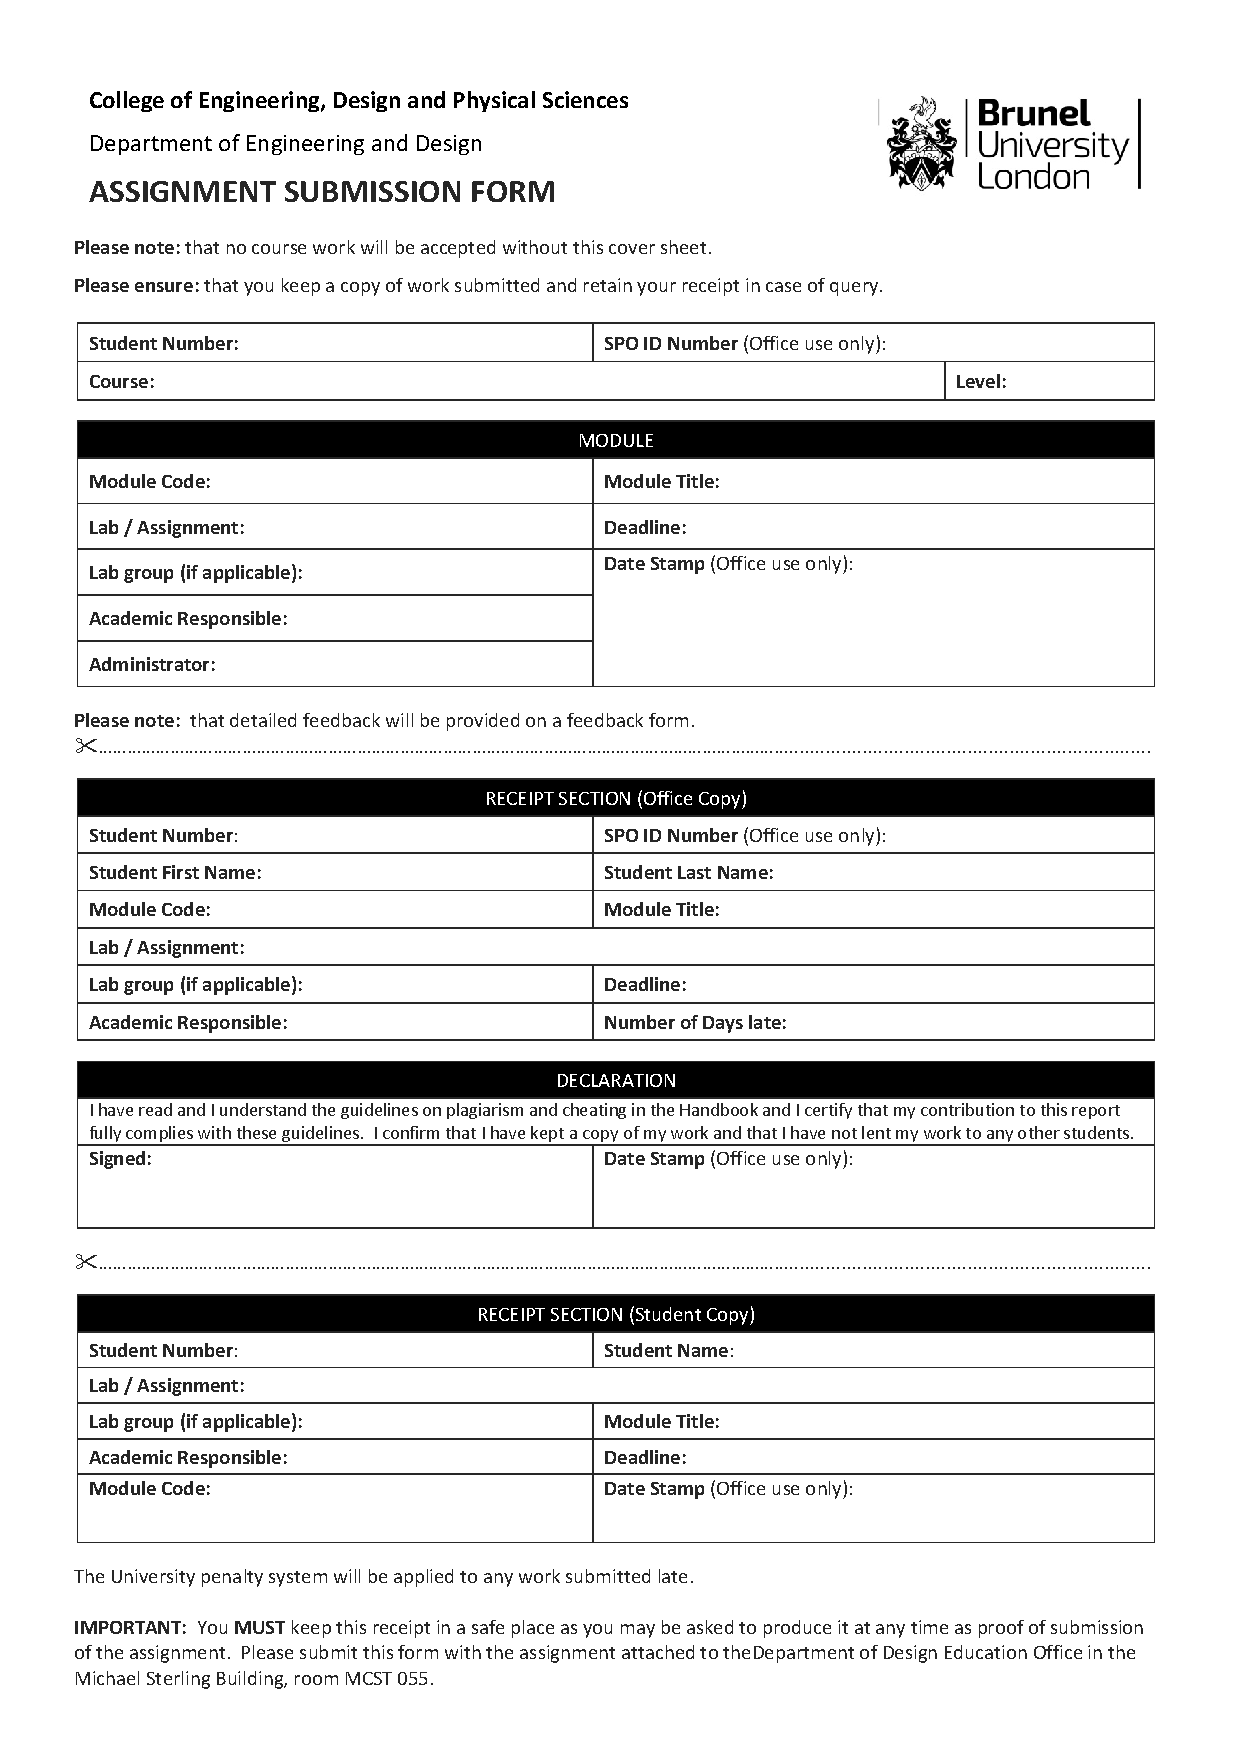
\includepdf{submission}
	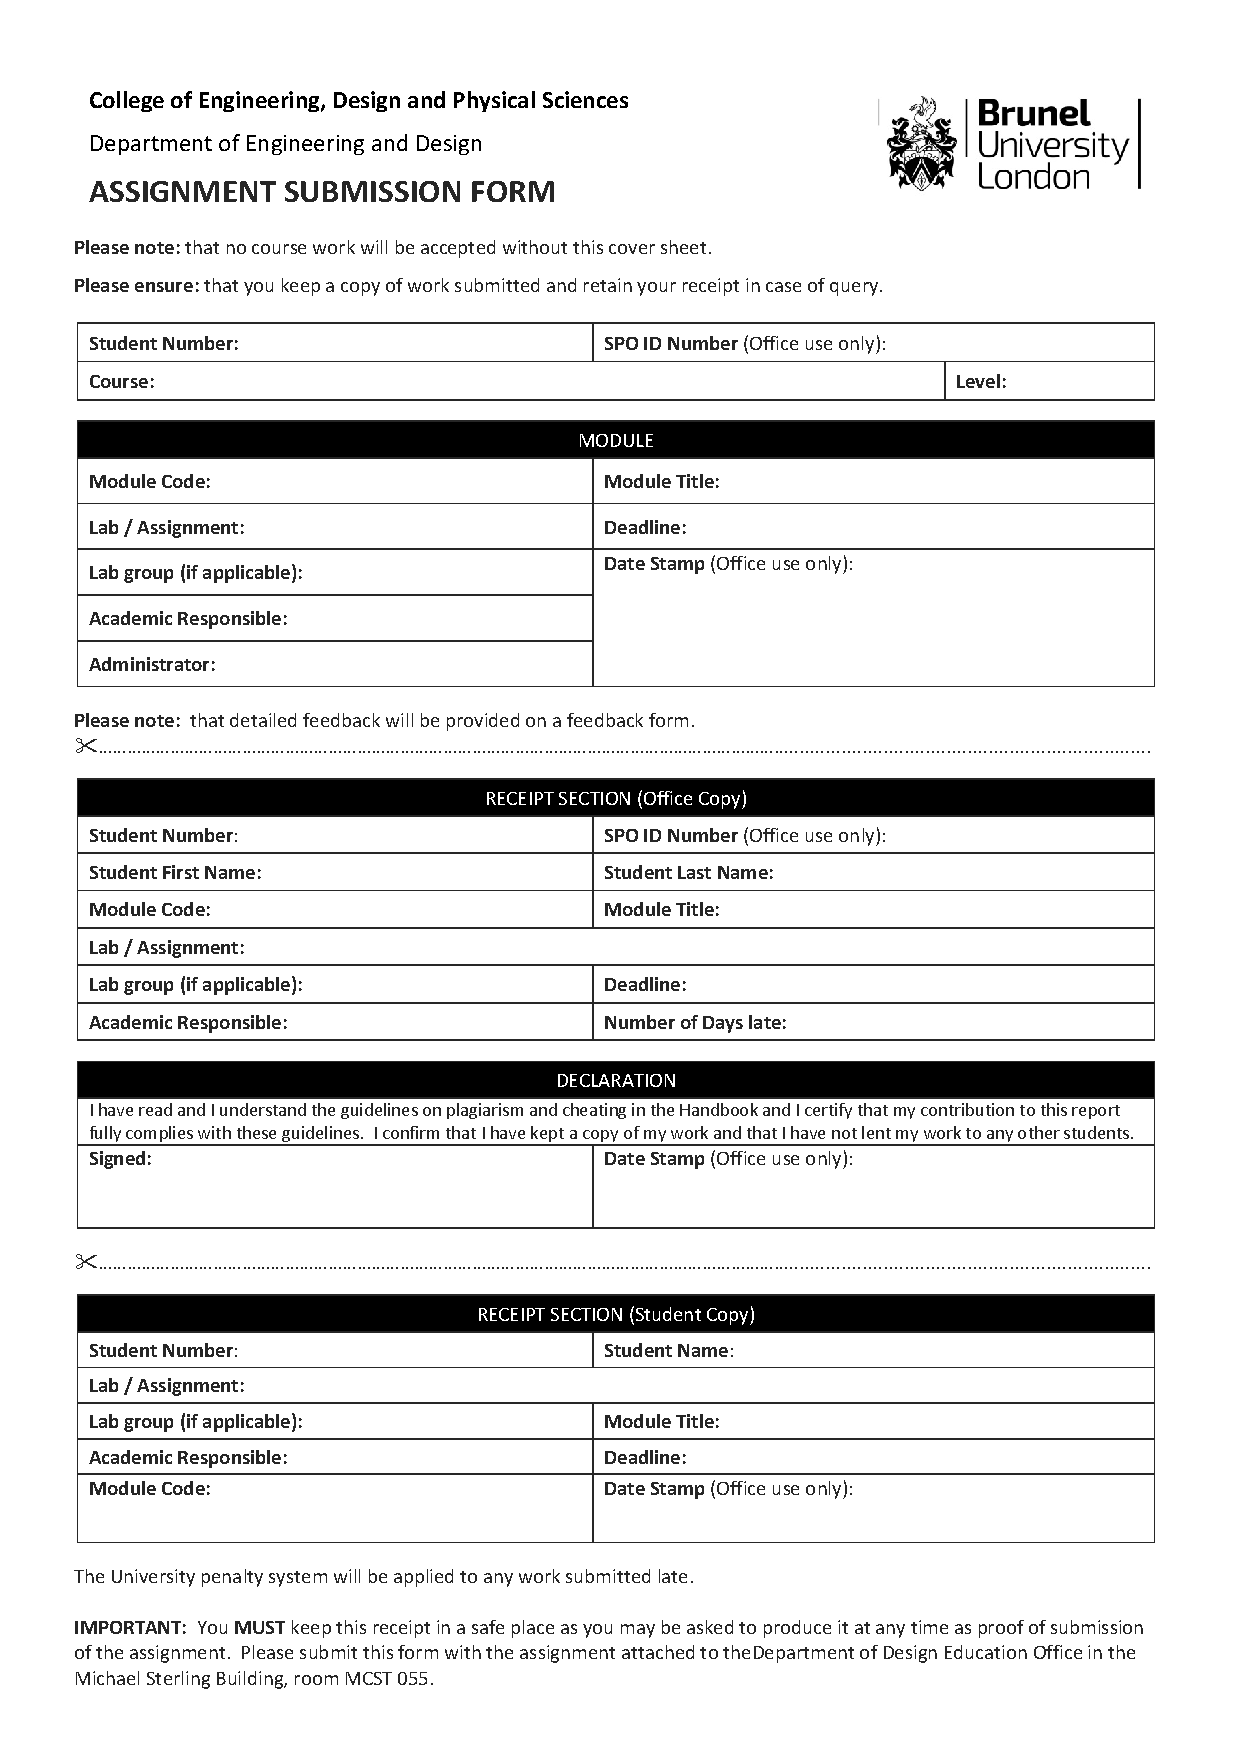
\includepdf{submission}
	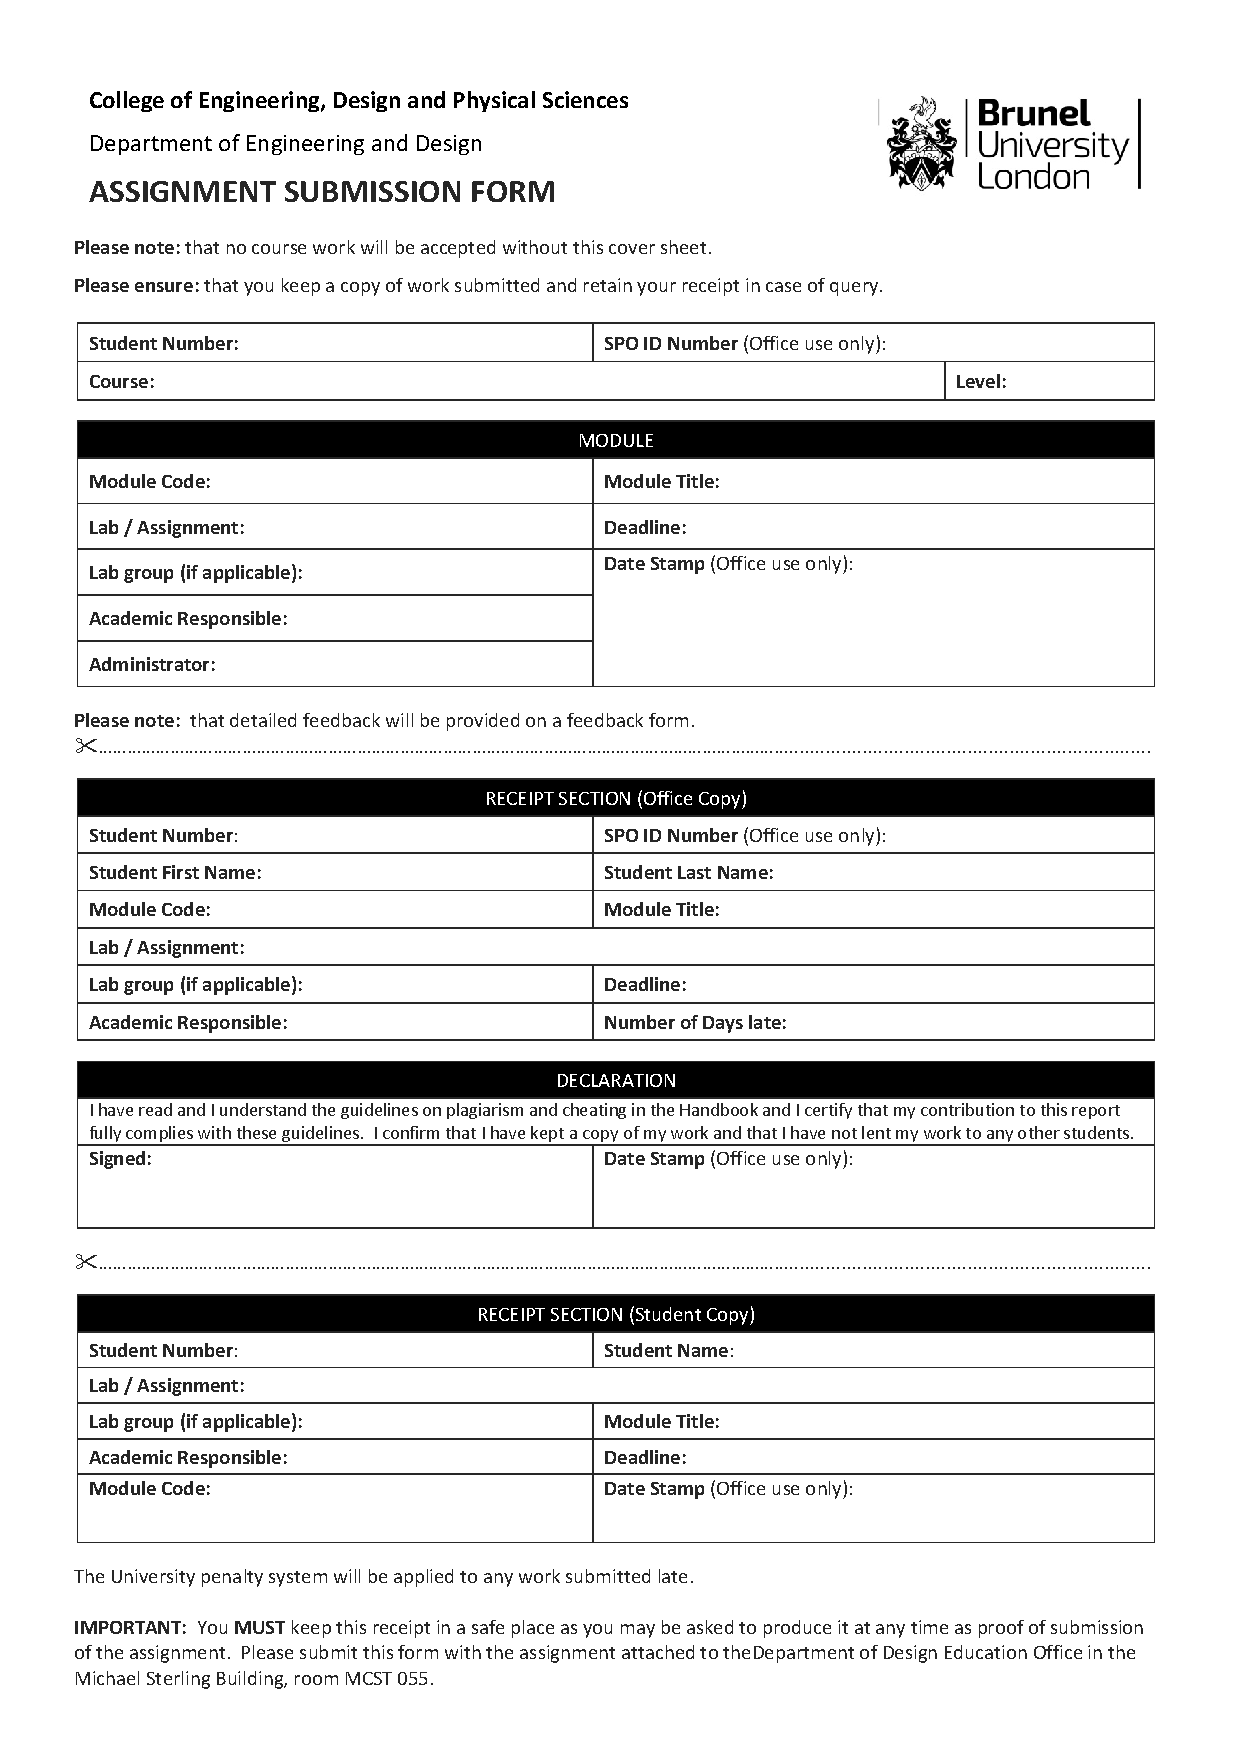
\includepdf{submission}
	%\include{chapters/ch-aa-vorspiel}
	%\include{chapters/ch-aa-zusfasg}
	% % Verzeichnisse
	\ihead[]{\leftmark} % links: Kapitel
	%\chead[\pagemark]{\pagemark} % mitte:
	\ohead[]{} % rechts: Section
	\automark[]{chapter}
	\tableofcontents
	\listoffigures
	\listoftables
	
	\ihead[]{\leftmark} % links: Kapitel
	%\chead[\pagemark]{\pagemark} % mitte:
	\ohead[]{} % rechts: Section
	\automark[]{chapter}
	
%	\input{abk-verzeichnis/abk}
	\clearpage
	%\lstlistoflistings % Verzeichnis f�r Code-Listing
\end{spacing}
% % %%%%%% Textteil (Eigentliche Arbeit)
\mainmatter
%
\ofoot[\pagemark\, \textbf{of \pageref*{LastPage}}]{\pagemark\, \textbf{of \pageref*{LastPage}}}


\chapter*{Abstract}
The aim of this work is to generate an application that starts a timer that measures the time of a certain activity by clapping into the hands. The timer is stopped by the repeated clapping and the time is saved together with a corresponding activity. This creates a history for the user in which he can see how long which activity was performed.
\\
The problem to be investigated is the proper detection of clapping noises. It must be possible to distinguish between background noises such as coughing or knocking. This presents a major challenge, as they are difficult to distinguish from a technical point of view.
\\
A large number of sound samples were recorded for clapping, tapping, coughing and speaking and the respective frequency spectrum was compared. In order to get a variation of the sounds different people have executed these tasks. In addition, various software tools are used to analyse the frequencies.
\\
The result of this work is that the analysed noises partly happen on the same frequencies. %Depending on who's making the noise. 
A distinction can therefore only be made in the duration of the tones. Using individual algorithms for this would become too complex, as many cases have to be covered. It therefore makes more sense to use pattern recognition frameworks. %However, they need a lot of test dates.
\\
When enough time is available, the use of pattern recognition frameworks makes the most sense. The devices that were used reliably detect the noises and the mathematical calculations are also possible without problems on the systems.
\chapter{Introduction}
\label{sec:org7d7a9e6}
\section{The Idea}
\label{sec:org0041e00}

The Digital Life Tracking App is designed to enable users to track their daily tasks and the time spent on them.
To make it more convenient to trigger an activity, the start and end of an activity may be triggered in different ways. 
Possible activation mechanisms could be:
\begin{itemize}
\item Two claps
\item moving the smartphone in a certain way (gestures)
\item activation based on GPS position
\item pressing a button
\end{itemize}

Users should be able to define their own activities and select an activation function from a list and assign it to one of their activities.
The user should then be able to display his history in form of charts.
A separate device (particle photon board) could also be used to trigger a specific activity.

\subsection{The Deep Dive}
\label{sec:orgf0412a9}
For the prototype in the context of the assigment we decided to focus mainly on the detection of double clapping as an activity trigger. From the original idea a concept for the following app was developed:

\begin{center}
	\textbf{{\Large Digital Life Tracking}}
\end{center}
\begin{figure}[H]
	\centering
	
\includegraphics[width=0.5\linewidth]{./imgs/appIcon.png}
\end{figure}
The app should allow a user to divide his daily routine into categories of activities and to measure the time required for each activity. This enables him to get an overview of his time invested in various activities.
\chapter{Data Analysis}
This chapter is about the analysis of the gathered data. The amplitudes of the signals are recorded and stored. The amplitudes alone say nothing about the signal, except how strong it is. Therefore it is necessary to transform it into the frequency domain via \textit{Fourier Transformation}\footnote{https://betterexplained.com/articles/an-interactive-guide-to-the-fourier-transform/}. This shows which frequencies are involved in the recordings. 
\section{First Prototype}
The first prototype for the detection of clapping was created with Particle's Photon Board. For this purpose the circuit was rebuilt as shown in Figure \ref{fig:photonBoard}\footnote{Source: MSc\_DCSE\_Assignment\_WS6\_Smartphone\_Sensing\_meets\_IoT\_2018\_final} and a test program was loaded with the corresponding Web IDE with which it is possible to collect initial data.
\begin{figure}[h]
	\centering
	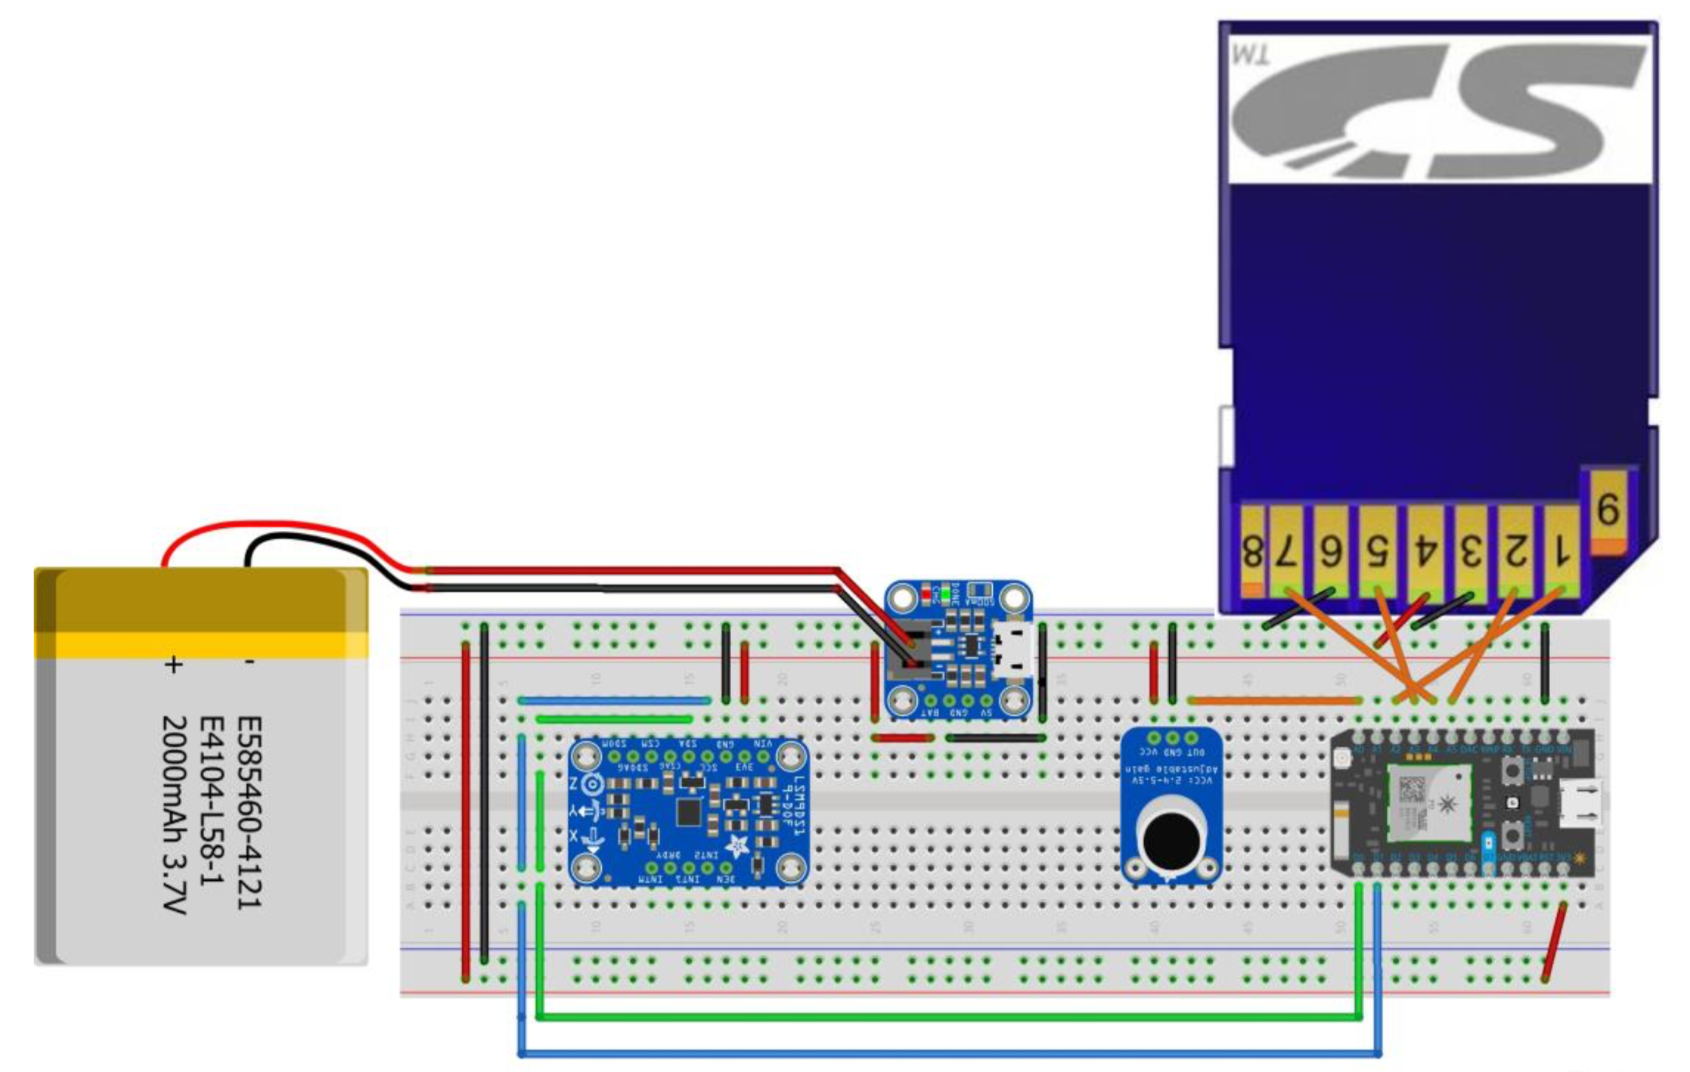
\includegraphics[width=.7\textwidth]{imgs/particleBoard}
	\caption{Particle's Photon Board}
	\label{fig:photonBoard}
\end{figure}
\newpage
The first six measurements were made at a sampling rate of 10Hz. By performing the Fast Fourier transformation on the collected amplitudes, it was possible to examine the amplitude spectrum. Figure \ref{fig:clapping10Hz} shows one result that captured the clapping correctly. This was not the case with every measurement. It can be said that 10Hz is too little for sampling, since possible clapping cannot be measured correctly or only partially in this way. A possible solution is therefore to increase the sampling rate to 1kHz. \newpage
\begin{figure}[h]
	\centering
	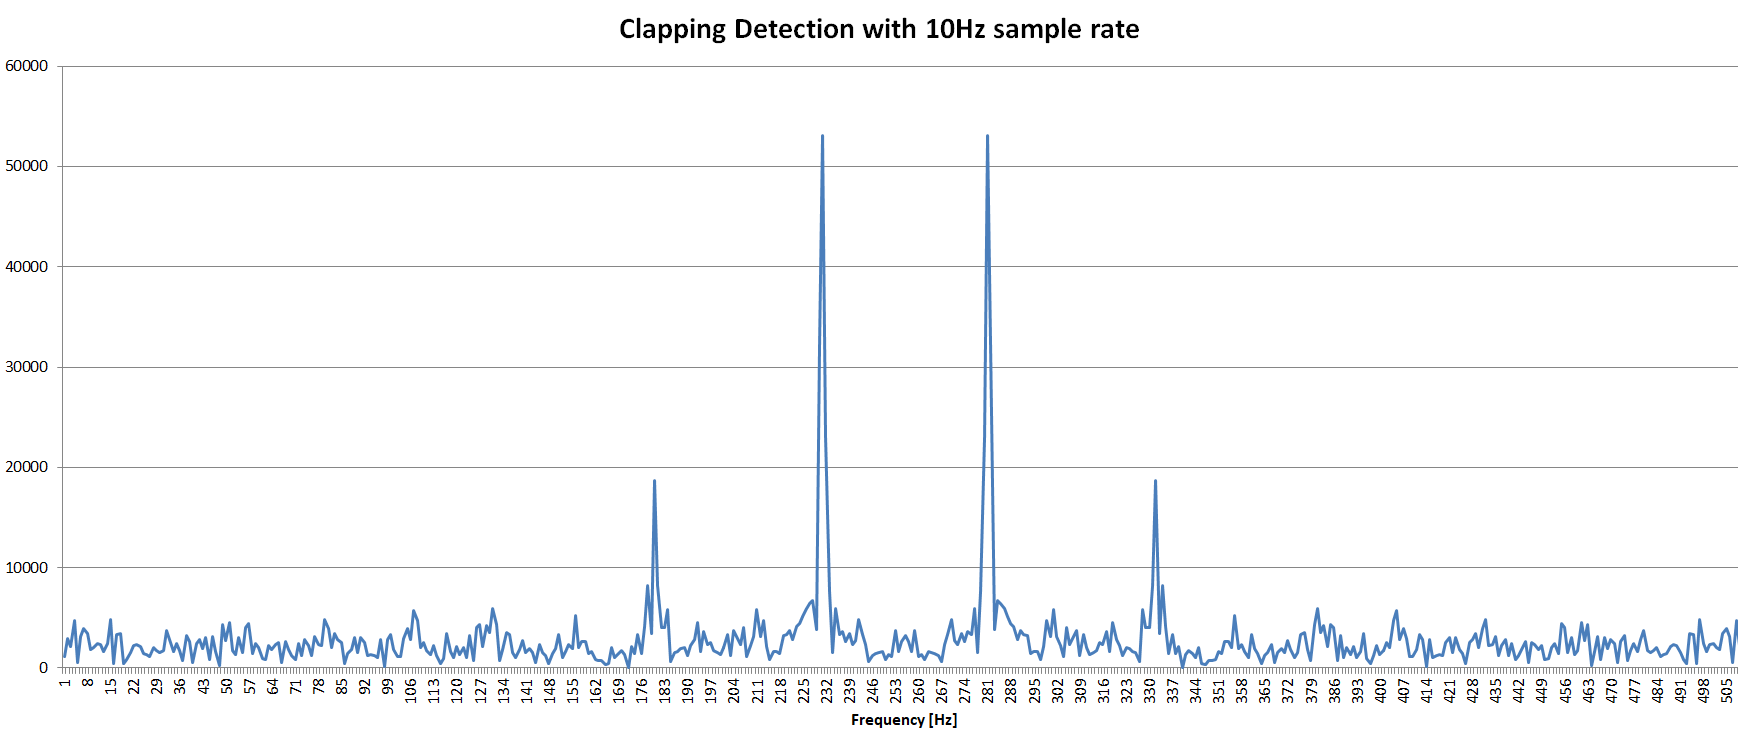
\includegraphics[width=\textwidth]{imgs/clapping10Hz}
	\caption{Amplitude Spectrum for Clapping with 10Hz sample rate}
	\label{fig:clapping10Hz}
\end{figure}
The following measurements have shown that writing to the SD card is too slow in each iteration, resulting in a reduced sampling rate of about 200Hz. It is therefore an idea to keep the data in the memory of the board until enough data has been collected to be written to the SD card at once. 
\\
By holding the data in the memory of the board, it is possible to obtain a higher sampling rate. However, the evaluation of the data is time-consuming, since they first have to be transferred from the SD card to a PC. With many measurements, the time adds up and makes the measurements no longer efficient. \\
Therefore, it makes more sense to use an Android smartphone with its microphone that can send the created CSV files directly, for example to the dropbox. Thus the data is quickly available for several persons and evaluations can be made directly. In addition to that a good debugger, exception handling, as well as reliable and sophisticated libraries for mathematical operations can be used. The implementation of the software for the Android phone and the used libraries are described in more detail in chapter \ref{sec:org11f3563}.
\section{Measurements with Android phone}
According to figure \ref{fig:clappingFreqBereich}\footnote{http://www.klangfuzzis.de/showthread.php?679817-Was-hat-in-etwa-wie-viel-hz} the frequency range of clapping lies between about 120Hz up  to 10kHz. If a 10kHz clapping shall be captured right, the sampling rate according to shannon's law\footnote{http://www.recordingblogs.com/wiki/nyquist-shannon-sampling-theorem} must be double the size of the measured signal. Therefore roughly 20kHz.
\begin{figure}[h]
	\centering
	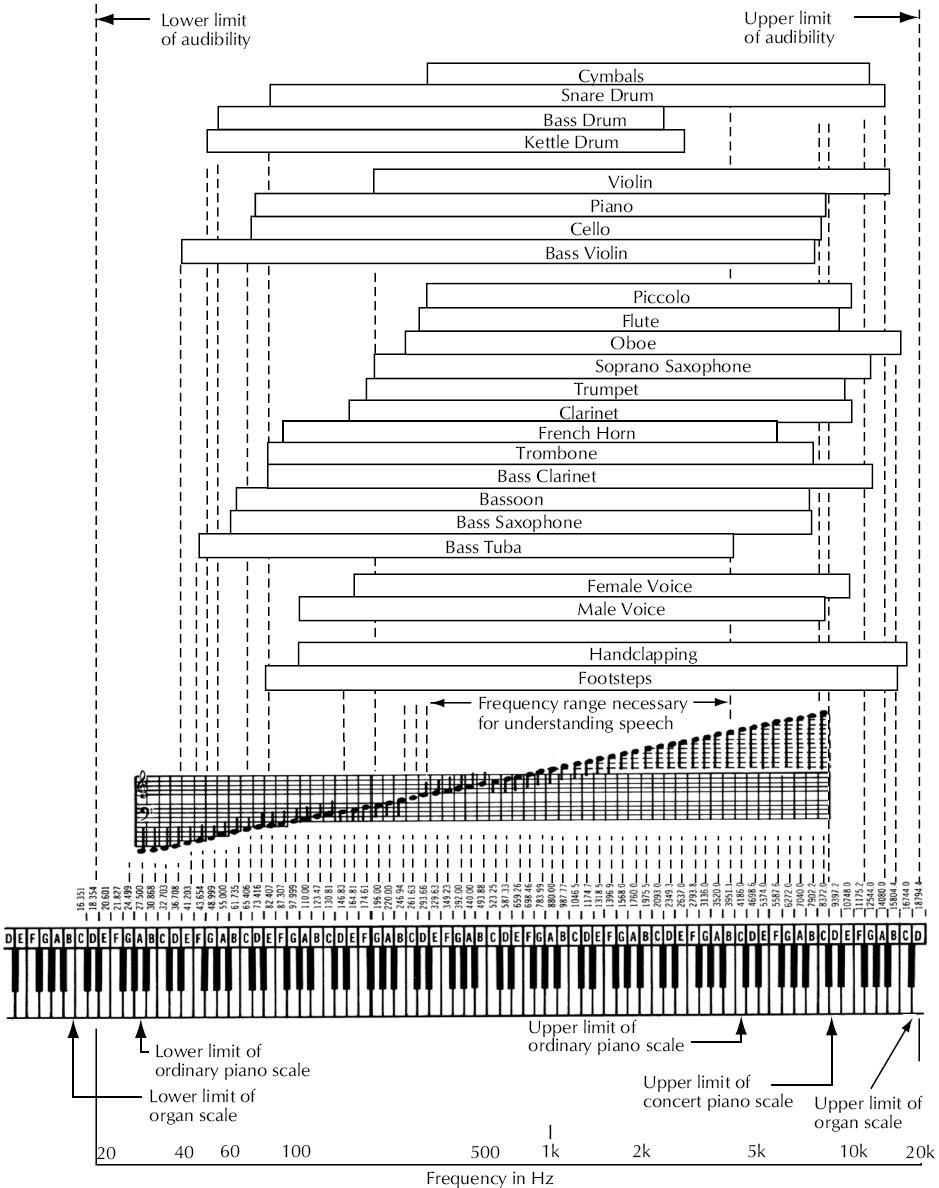
\includegraphics[width=.9\textwidth, trim={0 0 0 5.4cm},clip]{imgs/clappingFreqBereich}
	\caption{Frequency range of clapping}
	\label{fig:clappingFreqBereich}
\end{figure}\\
The first measurements with a sample rate of 22kHz generated the following figure (Figure \ref{fig:clappingAndroid}). Compared to Figure \ref{fig:clapping10Hz}, which shows the signal from the Particle Board, it can be said that the values for the frequency do not match (Table \ref{tab:comparisonParticleAndroid}). This is logical, since the range of the clapping is large. It was tried to perform a nearly similar clapping to retrieve almost identical data. Since this was not the case, an idea was to check the Android Software, if the data was calculated and transformed correctly.\\
\begin{table}[h]
	\centering
	\begin{tabular}{|l|l|}
		\hline
		\textbf{Particle} & \textbf{Android} \\
		\hline
		230Hz & 160Hz\\
		\hline
	\end{tabular}
\caption{Comparison clapping frequency of Particle Board and Android device}
\label{tab:comparisonParticleAndroid}
\end{table}
\begin{figure}[h]
	\centering
	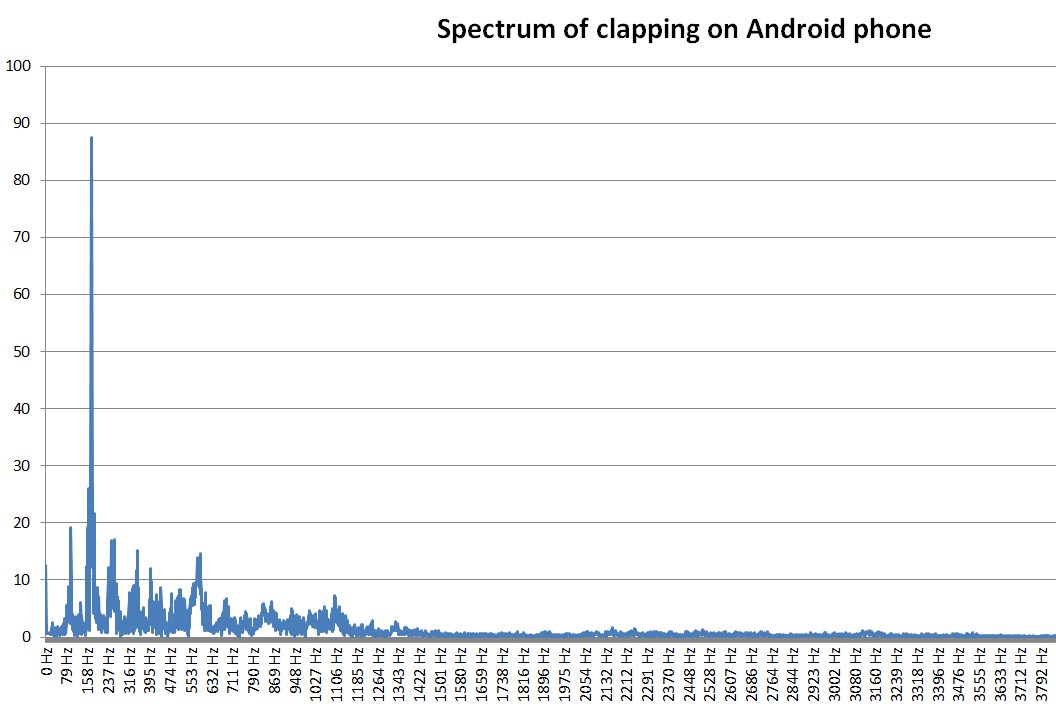
\includegraphics[width=\textwidth]{imgs/clappingAndroid}
	\caption{Amplitude Spectrum for Clapping with Android device}
	\label{fig:clappingAndroid}
\end{figure}\\
For this reason, the check of the calculations is done with another tool called iSpectrum, which can be installed on a MacBook. This makes it possible to collect live data from the laptops microphone to view the spectrum. \\
In order to compare the iSpectrum software and the Android device, a reliable source is needed that provides values for a specific frequency. The idea is to take a sound example and play it to both systems. This makes it possible to observe which values match the frequency.
\\
Instead of a single sound file, a video is used for testing, which plays all frequencies in the audible range of the human ear. This video is called \textbf{20Hz to 20kHz (Human Audio Spectrum)}\footnote{https://www.youtube.com/watch?v=qNf9nzvnd1k} and emits an increasing frequency from 20Hz to 20kHz. It is thus possible to see whether the values are correctly interpreted with different frequencies in the Android device.
\\
As figures \ref{fig:1200HzAndroid} and \ref{fig:1200HziSpectrum} show, the tested frequency of 1200Hz is reliably detected by both systems. Live testing with iSpectrum makes it very convenient to make clapping and other noises visible. Therefore, different sounds were tried out to see what the spectrum looks like.
\begin{figure}[h]
	\centering
	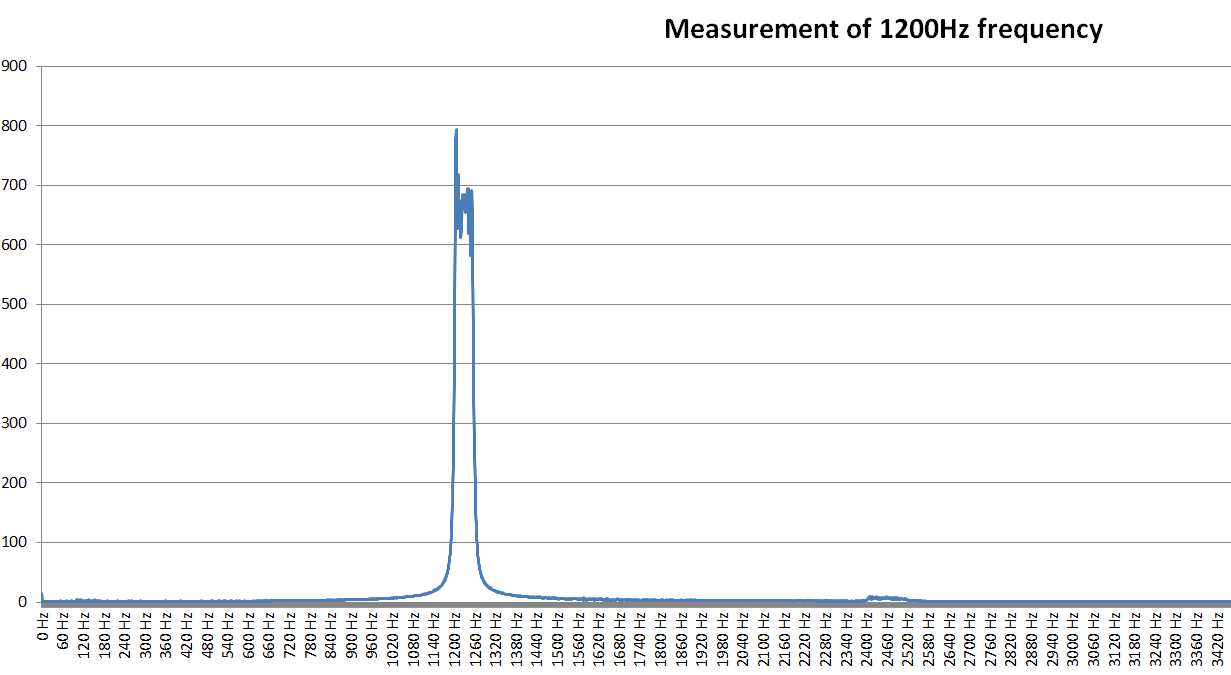
\includegraphics[width=.9\textwidth]{imgs/yt1200Hz}
	\caption{Amplitude Spectrum for 1200Hz (Android device)}
	\label{fig:1200HzAndroid}
\end{figure}
\newpage
\begin{figure}[h]
	\centering
	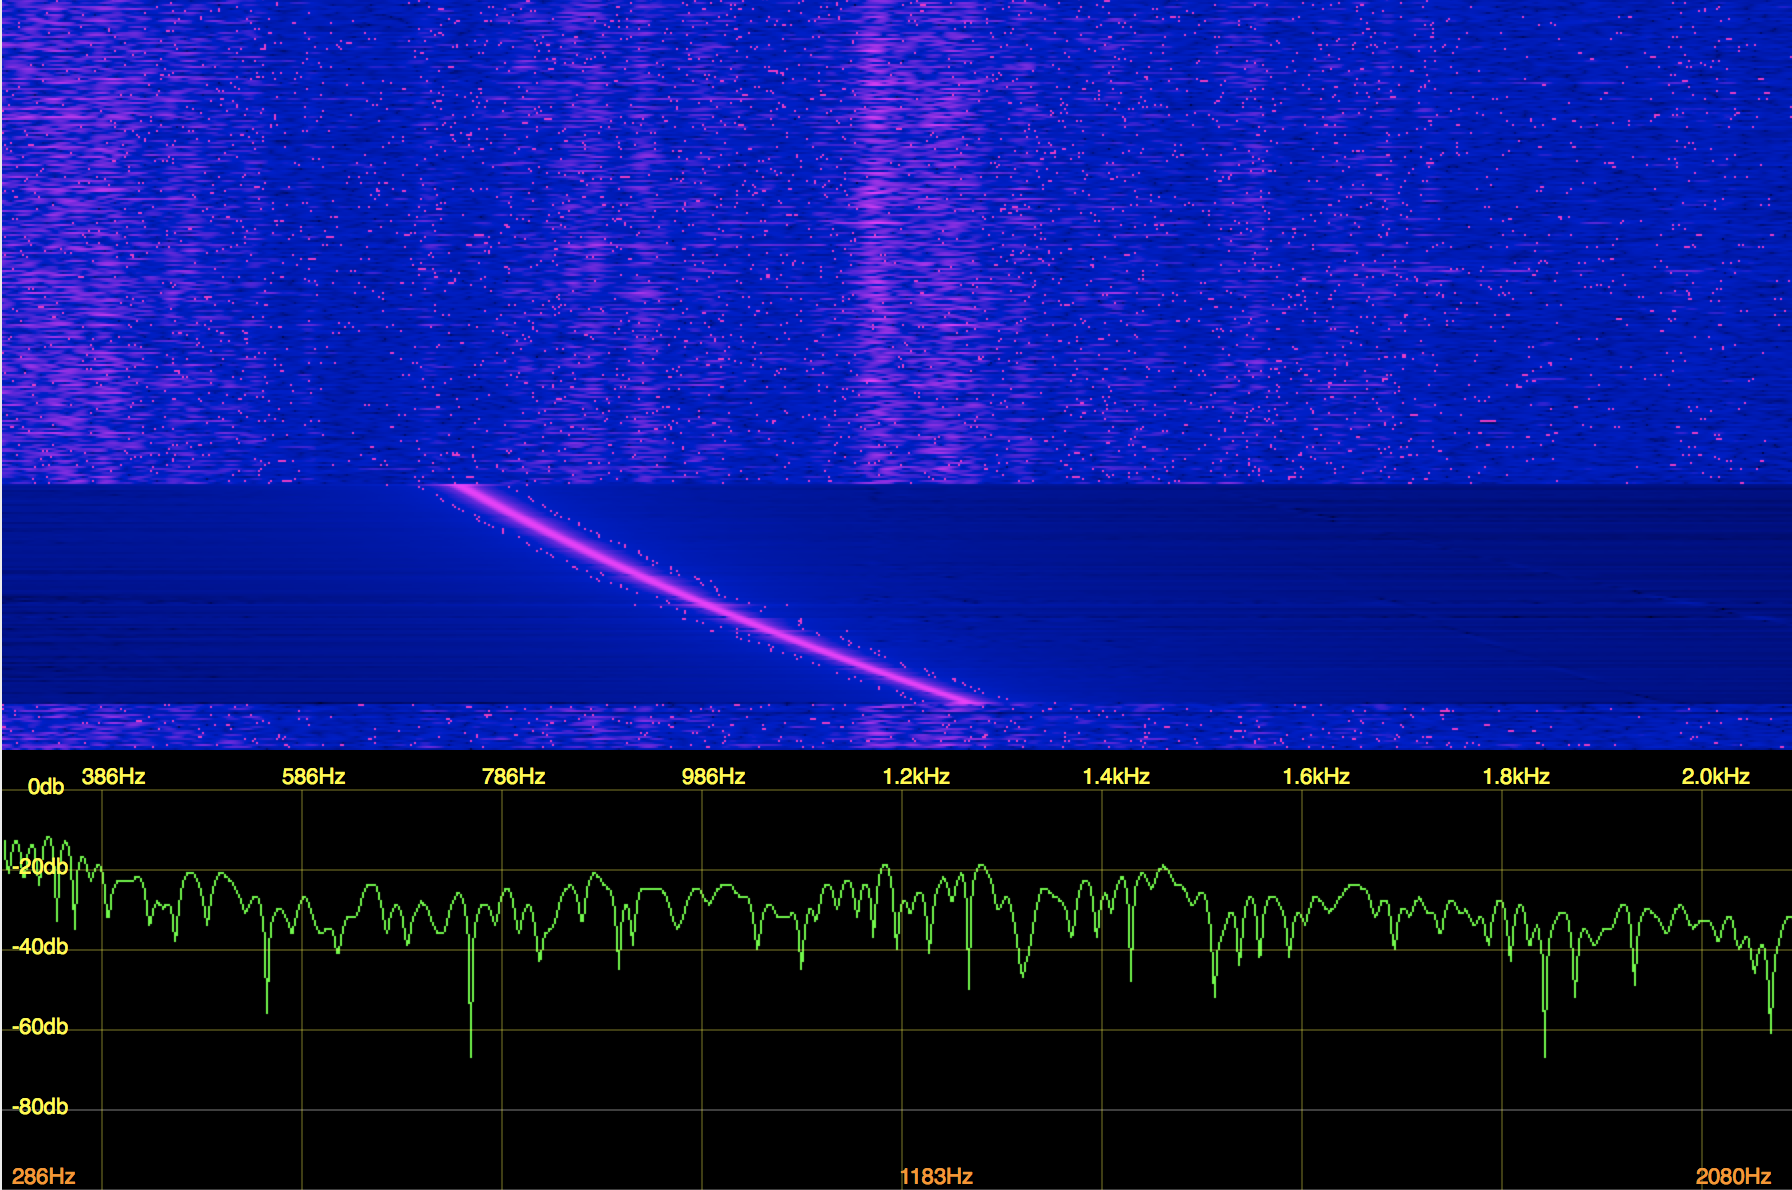
\includegraphics[width=.8\textwidth]{imgs/iSpectrum1200Hz}
	\caption{Amplitude Spectrum from 750Hz to 1200Hz (iSpectrum)}
	\label{fig:1200HziSpectrum}
\end{figure}
The yellow circle in Figure \ref{fig:clappingKnocking} shows the clapping in a small room. The three sounds detected, which have a green frame, are knocking on the table. It can be seen that these noises occur in different frequency ranges. The clapping echoes a little and the knocking stops abruptly. However, each clapping or tapping can be different from person to person, depending on how the clapping or tapping is performed, or where the person is. Further measurements with various test subjects have shown this. Figure \ref{fig:clappingE2} shows clapping from a test person in a big room. It can be obtained, that the clap has more echo in a big room compared to a small room. A distinction between clapping to other sounds could possibly be made with the duration of the echo.
\newpage
\begin{figure}[h]
	\centering
	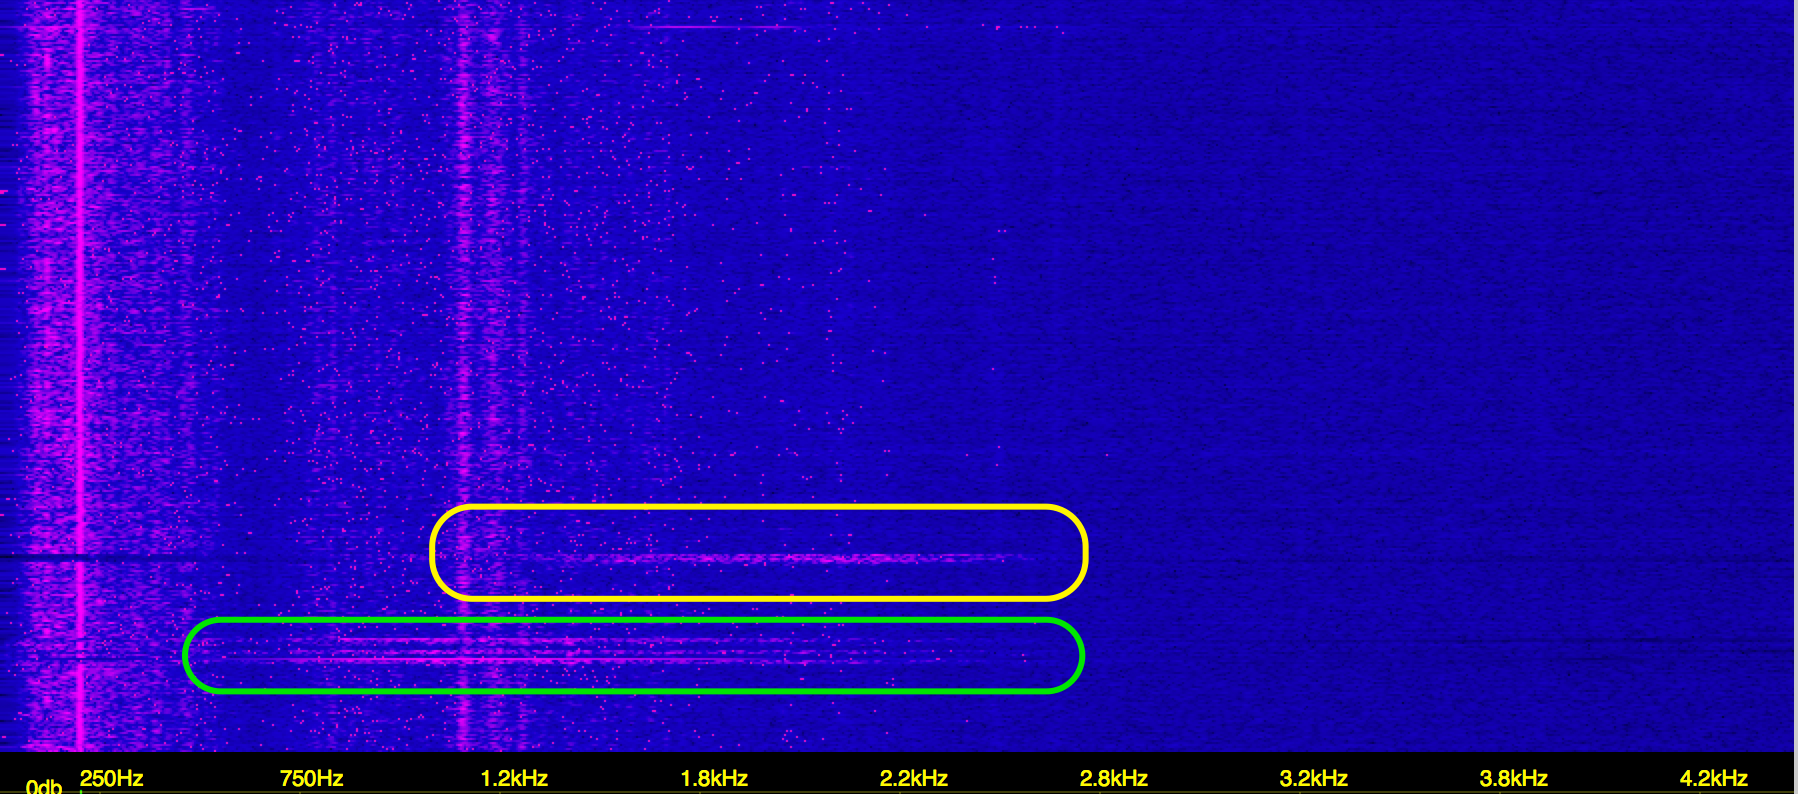
\includegraphics[width=\textwidth, trim={0 0 2cm 5cm},clip]{imgs/iSpectrumClappingKnocking}
	\caption{Spectrum of clapping and knocking}
	\label{fig:clappingKnocking}
\end{figure}
\begin{figure}[h]
	\centering
	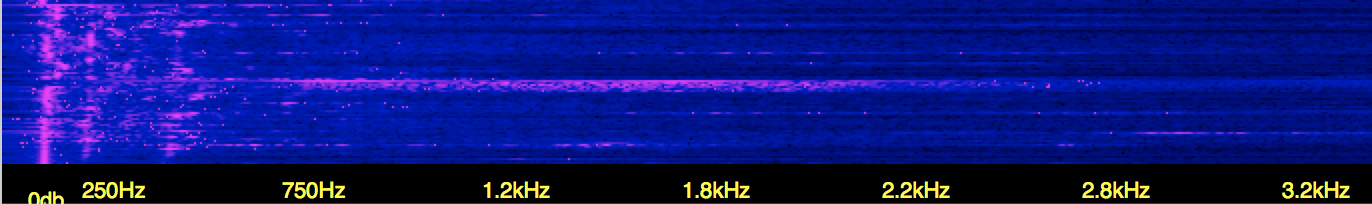
\includegraphics[width=\textwidth]{imgs/iSpectrumClappingE2}
	\caption{Spectrum of clapping in a big room}
	\label{fig:clappingE2}
\end{figure}
\section{Generated insights}
So far, the tests have shown that the clapping is in the range of 750Hz to 3kHz very consistently. That means that the first measurements with 10Hz and 1kHz are not usable, since according to Shannon's law it is not possible to measure this high frequencies with that small sample rate. That is why the first assumptions are completely wrong. Only the measurements with the Android device with a sampling rate of 22kHz provided clearer and more consistent results. Another assumption is that the measurements in Figure \ref{fig:clappingAndroid} give a false impression, since the strongest frequency is in the range around 160Hz. It is possible that the accumulated ambient noise has a higher amplitude than the clapping. This means that the frequency for the clapping is not displayed with a high amplitude. A possible solution for this scenario is to use a digital filter to capture and display only the frequencies of the clapping range. One filter of interest in this case would be the bandpass filter\footnote{https://www.electronics-tutorials.ws/filter/filter\_4.html}, which provides exactly the needed behaviour. The band can therefore be limited from 700Hz to 3kHz.
\\
It is of course very complicated to evaluate every single signal to determine if it is a clap. A single algorithm is therefore not capable of analyzing a wide range of clap frequencies. Therefore it makes sense to evaluate the filtered data with a neural network. However, it should be noted that it takes a lot of training to get a reliable data analysis. This means that many thousands of clap patterns must first be recorded in order to give the neural network the possibility to interpret the clap correctly. TensorFlow\footnote{https://www.tensorflow.org} offers a widely used open source framework for machine learning and provides a good solution strategy for analysing clap signals.
\chapter{Second Prototype (Android)}
\label{sec:org11f3563}

\section{Research for clap detection in android}
\label{sec:orgc78ecb4}
Java is known to have many open source libraries. For the processing of audio
signals, the open source library Tarsos\footnote{https://github.com/JorenSix/TarsosDSP} was a good choice. Among other things, this offers a
ready-made percussion detection which enables to detect sudden peaks in a
frequency. However, Tarsos also offers more basic functionalities, such as
transforming an audio signal into the frequency domain using Fast Fourier
Transformation.

In order to implement and test the necessary functionality for the state machine
and the UI, the percussions detection from Tarsos was initially used to detect a
loud noise.

\section{Implementation for data analysis}
\label{sec:org29c2ba8}
Some code was soley written for getting data out of the app and was removed 
later for the final app.

\subsection{Google Drive}
\label{sec:orgfdfd3aa}
When working on the first prototype with the Particle Photon Board, the
roundtrip time required to get the data from the board to a PC, where we can
analyze it, was particularly noticeable. For this reason, an automatic upload of
the CSV data to Google Drive has been implemented. This made it possible to
quickly transfer all recorded data to a central location and analyze it from
there on a PC.
\subsection{CSV Button}
\label{sec:orgcc3314e}
Another functionality that was only necessary for the initial phase is the
recording of the audio signal for a certain period of time and afterwards
writing the transformed (FFT) data into a CSV file.

An extra button was added to the page, which adds a new AudioProcessor to the
AudioDispatcher, which then writes the data to the mobile phone. The existing
CSVWriter class was used and adapted for this.

Unfortunately it turned out that you can't call the method
AudioDispatcherFactory from the Default Microphone twice to run two dispatchers with
different buffer sizes at the same time. For the recording of test data a longer
period of time is useful over which the FFT is then applied. A buffer size of
3*sampling size was needed, to allow 3 seconds of audio recording per test. For
real application, however, shorter periods of time are needed to detect a double
clap and to keep the delay of the detection small.


\section{Implementation}
\label{sec:org7c927b3}
\subsection{Clap Detector}

The ClapDetector creates a new AudioDispatcher with a buffer size of 1024 bytes and a sample rate of 20kh and registers itself as AudioProcessor.
Thus, the AudioDispatcher calls the AudioProcessor Process Handler with 1024 amplitude values every 0.02 seconds.
For each time period, a Fast Fourier transformation is created using the Tarsos library. The number of peaks is counted for each new frequency spectrum.
The peaks are detected by iterating over each frequency and calculating the decibel values for each magnitude. The decibel value is then compared with a fixed threshold.
All decibel values that exceed the threshold are counted. The ClapDetector stores only the last two PeakCounter values.
To detect a clap, the second last peak counter must be smaller than the last and the current one smaller than the last.
If this is the case, an increase and decrease has been detected in several frequency ranges and the handler is called.


\subsection{State-machine}
\label{sec:orgd3a5b2d}
A state machine was implemented to represent the different states of the app.
The following diagram shows the implemented state machine.

\begin{figure}[H]
	\centering
	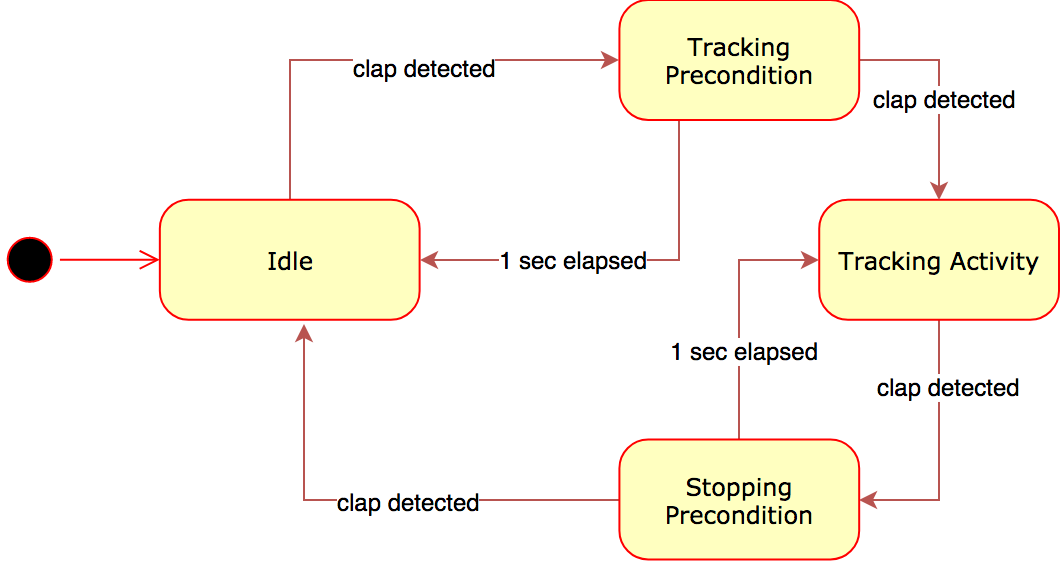
\includegraphics[width=1.0\linewidth]{./imgs/statemachine.png}
	\caption{UML State Chart Diagram for the state machine}
	\label{statemachine}
\end{figure}

There are a total of four states in which the app can be in. 
\begin{itemize}
\item Idle: The initial state when starting the app and the state after an activity tracking has been completed.
\item StartPrecondition: If the app is in the idle state and a clap is detected, the state machine switches to this state. When switching to this state, a timer is started which defines the time window in which the second clap must occur in order to switch the state to TrackingActivity. If the timer expires before another clap is detected, the state machine switches back to the idle state.
\item TrackingActivity: After a second clap is detected while the timer of the start precondition has not yet elapsed, the state machine changes to this state and starts capturing the time by saving a time stamp.
\item StoppingPrecondition: If the state machine is in the TrackingActivity state and a clap occurs, then the state machine switches to this state, which behaves in the same way as the StartingPrecondition, except that on a successful second clap, it changes to the idle state and the tracking of the current activity is ended.
\end{itemize}

\subsection{Architecture}
\label{sec:org393d659}
This Chapter describes the architecture for the Digital Life Tracking App. The following figure \ref{class-diagram} shows the class diagram with the most important classes:

\begin{figure}[H]
	\centering
	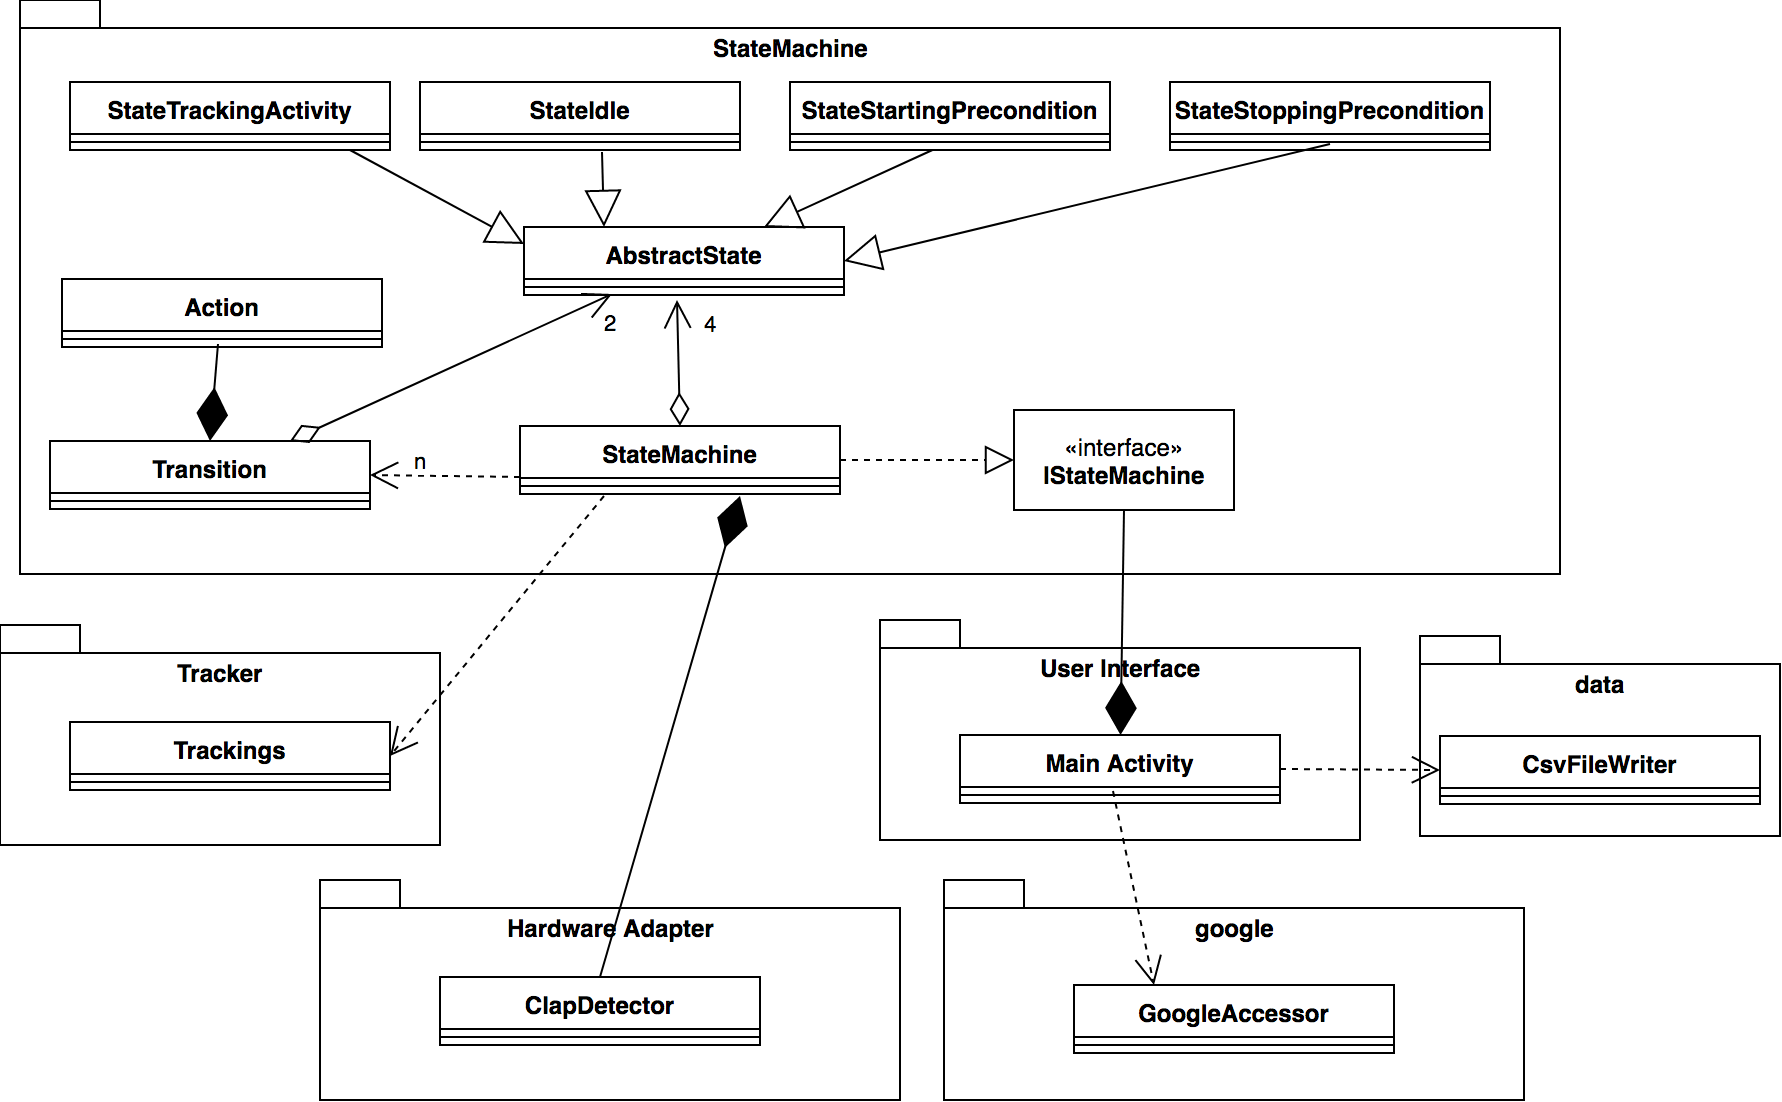
\includegraphics[width=1.0\linewidth]{./imgs/classUML.png}
	\caption{UML Class Diagram}
	\label{class-diagram}
\end{figure}

\subsubsection{StateMachine}
\label{sec:org9ea54c6}

The state machine presented in the previous chapter takes care of the logic 
of the app and switches back and forth between states when registering the corresponding event. 
The Statemachine class is the center of the package of the same name and performs the tasks described in the previous chapter.
It holds instances of all four states and a configuration of all possible transitions between the individual states.
Each transition in the configuration is also linked to an action that determines the event that triggers 
the transition. Each transition also defines the previous state and the next state.
When a transition is triggered, other operations are also executed that either adapt UI elements to the new 
state or execute other functions that are important for parts of the business logic.

\subsubsection{Hardware Adapter}
\label{sec:org0a1c43f}
The hardware adapter package includes the ClapDetector class, which uses the SmartPhone's microphone to listen 
for ambient sounds and tries to detect a clap from the recorded frequencies. When a clap is detected, 
a handler is triggered in the state machine. This triggers a transition between two states in the state machine.
This is illustrated in figure \ref{statemachine}.

\subsubsection{Tracker}
\label{sec:orgd2cdde2}

One of the operations triggered by the transitions in the state machine is to start or stop the tracker, 
which stores the activities of the user together with the measured times in a list.

\subsubsection{User Interface}
\label{sec:org2938786}

The User Interface package contains the main activity of the app, which initializes the other functions of 
the program including the state machine. The goal was that the Main Activity class should contain as little 
business logic as possible. The business logic has been implemented almost completely in the state machine. 
If possible, the class should only provide and control the UI elements of the app. It also controls the permissions 
request to the user, which the user must give in order for the apps to work properly.

\subsubsection{Google}
\label{sec:org3d3dca0}
This package contains the GoogleAccessor class, which was initially designed to upload the test data stored on the 
smartphone via the CSVWriter class to the Google Cloud. Once enough data has been collected, this functionality has 
been disabled for the release of the app. The reason for this was that access to the cloud required signed APK, 
which had nothing to do with the pure functionality of the app. Commenting out the code of this feature should 
avoid unnecessary problems when starting the app.

\subsubsection{Data}
\label{sec:orgdeb052b}
The data package contains the CsvFileWriter class, which stores the frequencies recorded by the ClapDetector in 
CSV files on the memory of the smartphone. This functionality was used during development to collect test data 
for later analysis.

\subsection{UI Design}
\label{sec:orgc19d2ea}
In order to make faster progress in the development of the app, a user interface was initially implemented, which was designed for the developers' tasks. The interface should display the transitions between the individual states of the state machine and the events in an output field as logs. The interface should also support the collection of test data that was later uploaded to the Google Cloud for analysis. 
\\\\
At the same time, a design for the future user interface was also created, which was intended to replace the development interface after completion of the basic functionalities of the app. The following figure \ref{mockups} shows mockups for both user interfaces:
\begin{figure}[H]
	\centering
	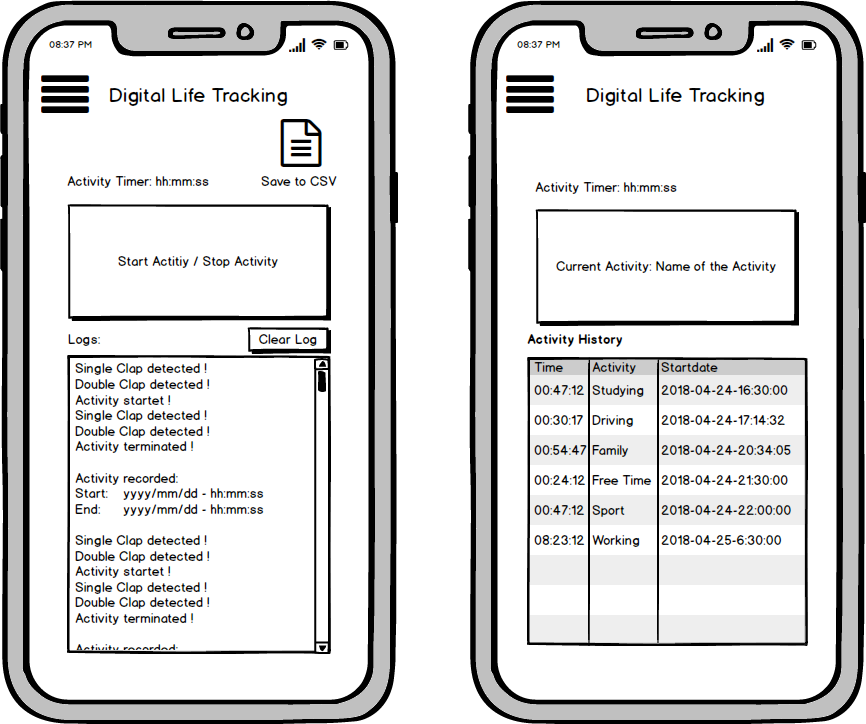
\includegraphics[width=1.0\linewidth]{./imgs/mock.png}
	\caption{Mockups for development UI (left) and for the final UI (right)}
	\label{mockups}
\end{figure}
The finished user interface should display a timer for the currently tracked activity and the name of the activity. In addition, it should display the last completed activities in a cronologically arranged list, whereby the name of the activity, the start time, as well as the duration of the activation should be visible.
\\
Since there was not enough time to implement the actual user interface during development later on, the app only has the development UI as it is currently available. Figure \ref{ui-screenshot} shows a screenshot of the actual development UI:
\begin{figure}[H]
	\centering
	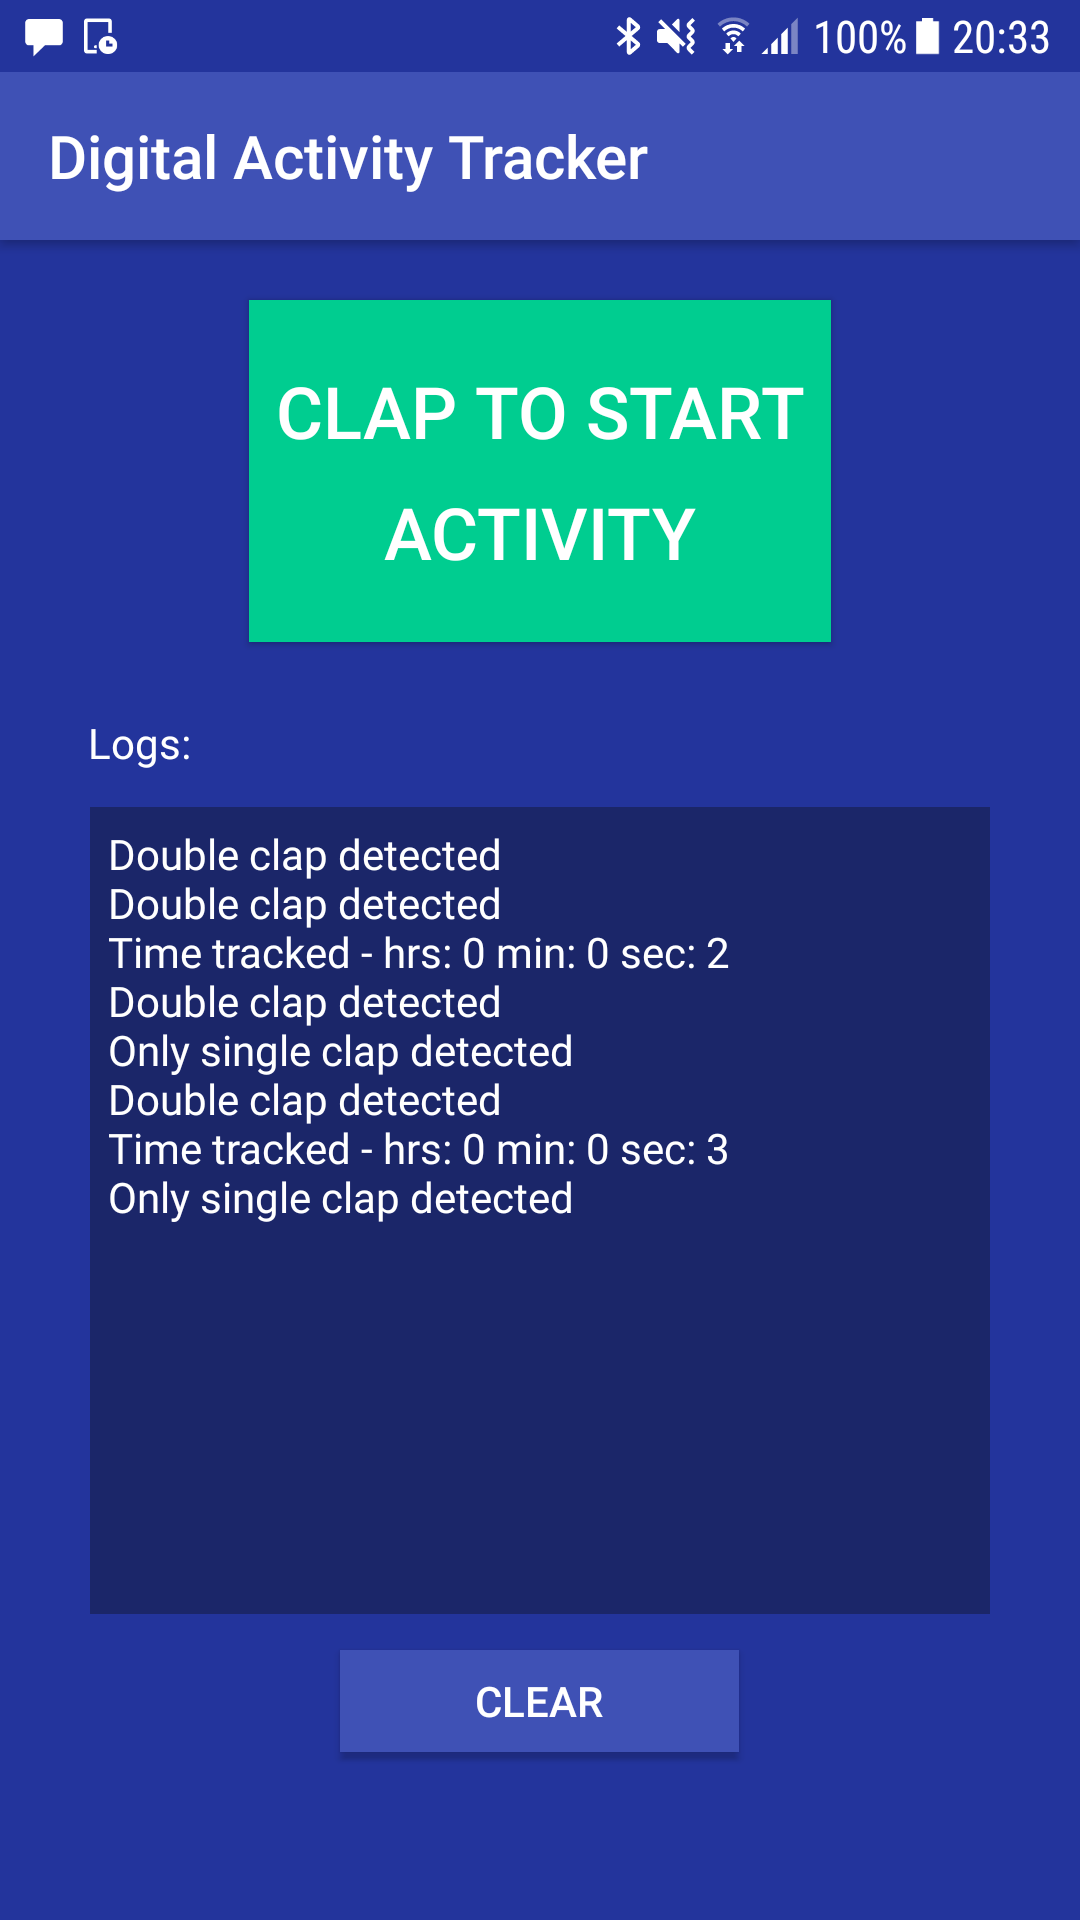
\includegraphics[width=0.5\linewidth]{./imgs/uiScreenshot.png}
	\caption{Screenshot of the development UI}
	\label{ui-screenshot}
\end{figure}
\chapter{Conclusion}

\section{Current State}


The current state of clap detection causes some false positives. 
Often voices are also recognized as clapping, or flicking with fingers or coughing.
Since there was not enough time to implement pattern recognition using a neural network, the app recognizes every pitch in a frequency range as a clap.

Frequently it happens to the user that when trying to clap twice, one of the claps is not loud enough because he has not hit his hands properly and therefore just
a single clap is detected.

If one examines the current state of the app for its usability, it is obvious that it would probably be quite unfavorable for the user experience if false positives ended the timer unintentionally, since the user would be currently busy with an activity and not immediately notice it.



\section{Project Outlook}
\label{sec:orgfa9fd4b}


To work on the problem further, some debugging functionality within the app would be good, so it would be faster to try different parameters instead of rebuilding the app over and over again.

Data analysis has shown that clapping is very difficult to detect. Compared to clapping, a clear pattern can be seen in the frequencies of a whistle sound. For the future of the app it might be better to detect a whistle instead of a clap to toggle the time tracking.

% % %%%%%% Literaturverzeichnis (darf im deutschen nicht in den Anhang!)
% Einfaches Literaturverzeichnis
%\input{chapters/ch-zz-bibEinfach}
% Literaturverzeichnis mit Bibtex
%\Urlmuskip=0mu plus 1mu\relax
%\ihead[]{\leftmark} % links: Kapitel
%\chead[\pagemark]{\pagemark} % mitte:
%\ohead[]{} % rechts: Section
%\automark[]{chapter}
%\raggedright
%\sloppy
%\ihead[]{}
%\bibliographystyle{unsrt}
%\bibliography{bib/bib}

% % %%%%%% Anhang
%\appendix
%\include{chapters/ch-zz-anhang}

% %  Inhalt ENDE %%%%%%%%%%%%%%%%%%%%%%%%%%%%%%%%%%%%%%%%%%%%%%%%%%%%%%%%%%
\end{document}
